In this section, we compare results of different adapted meshes obtained from three adaptive strategies mentioned above. 
We compare different quantities of interest. 
A comparison of force response in the form of normalized lift and drag forces is shown in Figures \ref{fig:lift_plot} and \ref{fig:drag_plot}, respectively. The normalized lift and drag matches up well for all the adapted meshes.

A comparison of spanwise vorticity for the different adapted meshes is shown in Figures \ref{fig:vorticity_195}, \ref{fig:vorticity_210} and \ref{fig:vorticity_270} for 3 phases of $\psi=210^\circ$, $\psi=225^\circ$ and $\psi=270^\circ$, respectively.
For $\psi=195^\circ$, as the airfoil is in the retreating phase, boundary layer roll-up is observed towards the geometric leading edge over the upper surface of the airfoil.
For the mesh based on zonal refinement, as we go from M0\_nz25 to Mza1\_nz50, the separation over the airfoil is well resolved, and finer flow scales/structures are visible on the adapted mesh.
Comparing Mza1\_nz50, Msa1\_nz50, and Mfa1\_nz50 meshes, we can see that the Msa1\_nz50 mesh (sizefield-based adapted mesh) does not capture the finer scales/structures as compared to the Mza1\_nz50 mesh, both over the airfoil surface and in the wake of the airfoil, i.e., flow structures are more diffused in the case of Msa1\_nz50.
On the other hand, the Mfa1\_nz50 mesh captures them well.

\begin{figure}[H]
\centering

\begin{subfigure}[b]{0.7\textwidth}
\centering
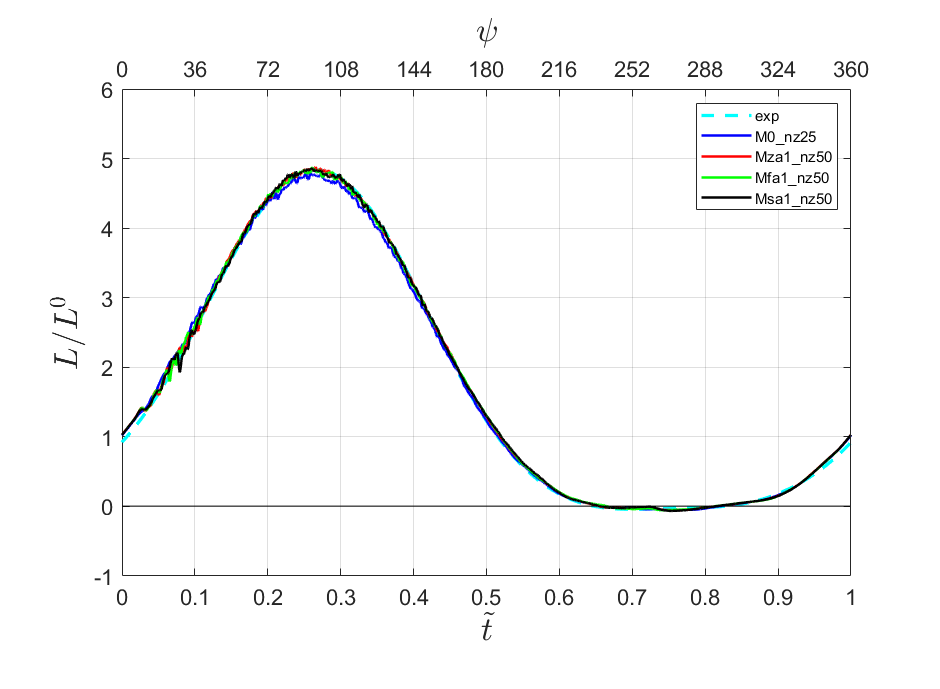
\includegraphics[width=1\textwidth]{figures/Results/Lift_adapt_strat.png}
\caption{Normalized lift}
\label{fig:lift_plot}
\end{subfigure}
\begin{subfigure}[b]{0.7\textwidth}
\centering
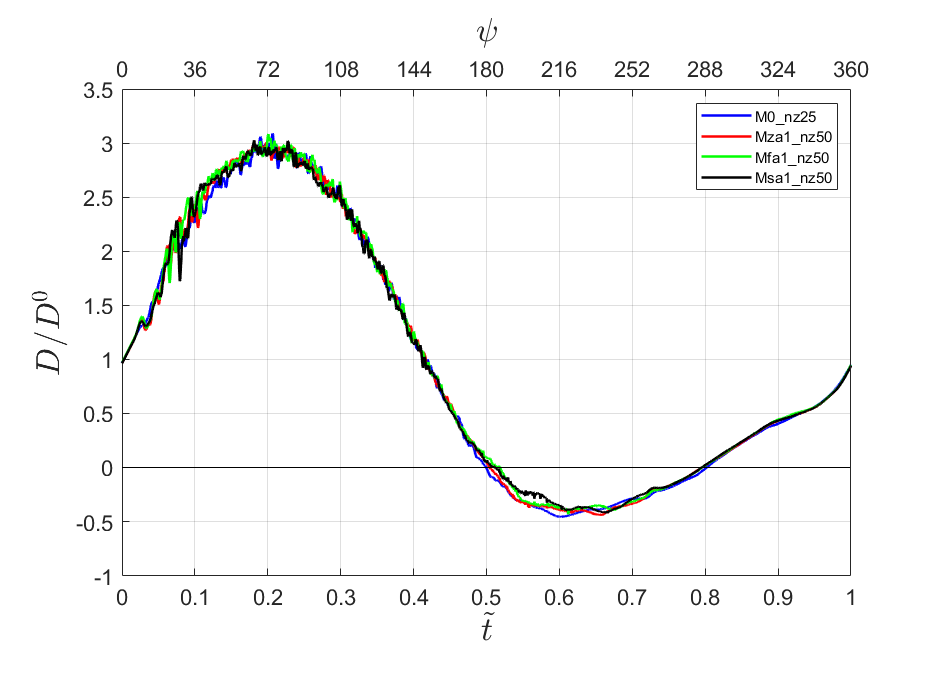
\includegraphics[width=1\textwidth]{figures/Results/Drag_adapt_strat.png}
\caption{Normalized drag}
\label{fig:drag_plot}
\end{subfigure}

\label{fig:force_response_adapt}
\caption{Normalized forces for different adaptive strategies/adapted meshes}
\end{figure}

%Next, we look at the location of the LEV core for different meshes in Figure \ref{fig:LEV_location}. Some differences in the LEV location for various phases are observed. LEV location for Ma1, FB, and hadapt meshes is similar in the beginning phases. Ma1 starts to deviate from FB and hadapt in the later phases. LEV location for FB and hadapt meshes start to match with Ma2 in the later phases, whereas M0 LEV location fluctuates around the other meshes. This however is still not conclusive as to which mesh performs better and a more quantitative study is needed.


%%\begin{figure}[H]
%\centering
%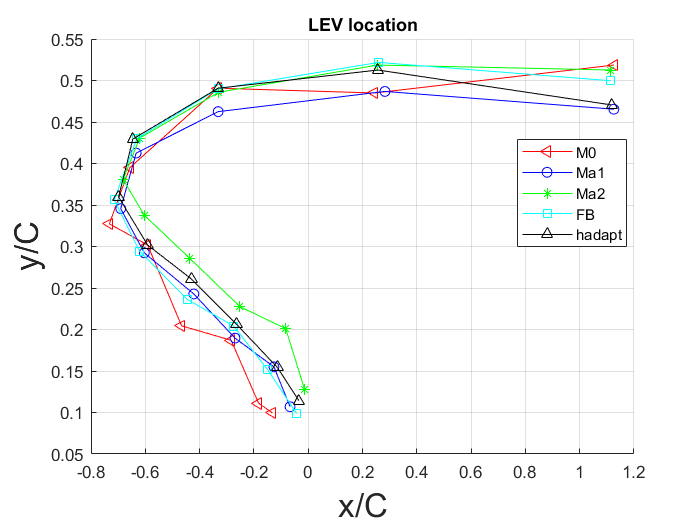
\includegraphics[width=0.7\textwidth]{figures/Results/LEV_location.png}
%\caption{LEV location for different meshes}
%\label{fig:LEV_location}
%\end{figure}
%%


For $\psi=210^\circ$, formation of LEV begins to take place, as we start to see the roll-up of separated shear layer near the geometric leading edge. 
At this phase, the differences in the flow structures resolved by the different meshes become more clear.
Similar to $\psi=195^\circ$, the Msa1\_nz50 mesh shows a relatively poor resolution of the finer flow structures as compared to the Mza1\_nz50 and Mfa1\_nz50 meshes.

For $\psi=270^\circ$, differences can be seen among different adapted meshes in the separated shear layer at the geometric leading edge of the airfoil, and in the LEV.
These are resolved better on the Mfa1\_nz50 and Mza1\_nz50 meshes. 
Recall that Mfa1\_nz50 is obtained using the feature-based mesh refinement designed to capture the LEV accurately, and has the same mesh resolution as Mza1\_nz50 along the path of the LEV. 
%Once again, shear layer is not well resolved for Msa1\_nz50 as compared to other refined/adapted meshes.

The relatively poor resolution of flow, with more diffused flow structures, observed for Msa1\_nz50 can be attributed to the variation in mesh sizes (even by a factor of 1.5 or 2) in crucial regions of interest, i.e., the mesh size is not uniform or even quasi-uniform in particular zones. In particular, this seem to have an adverse effect in regions with turbulence.

\begin{figure}[H]
\centering
\begin{subfigure}[b]{0.475\textwidth}
\centering
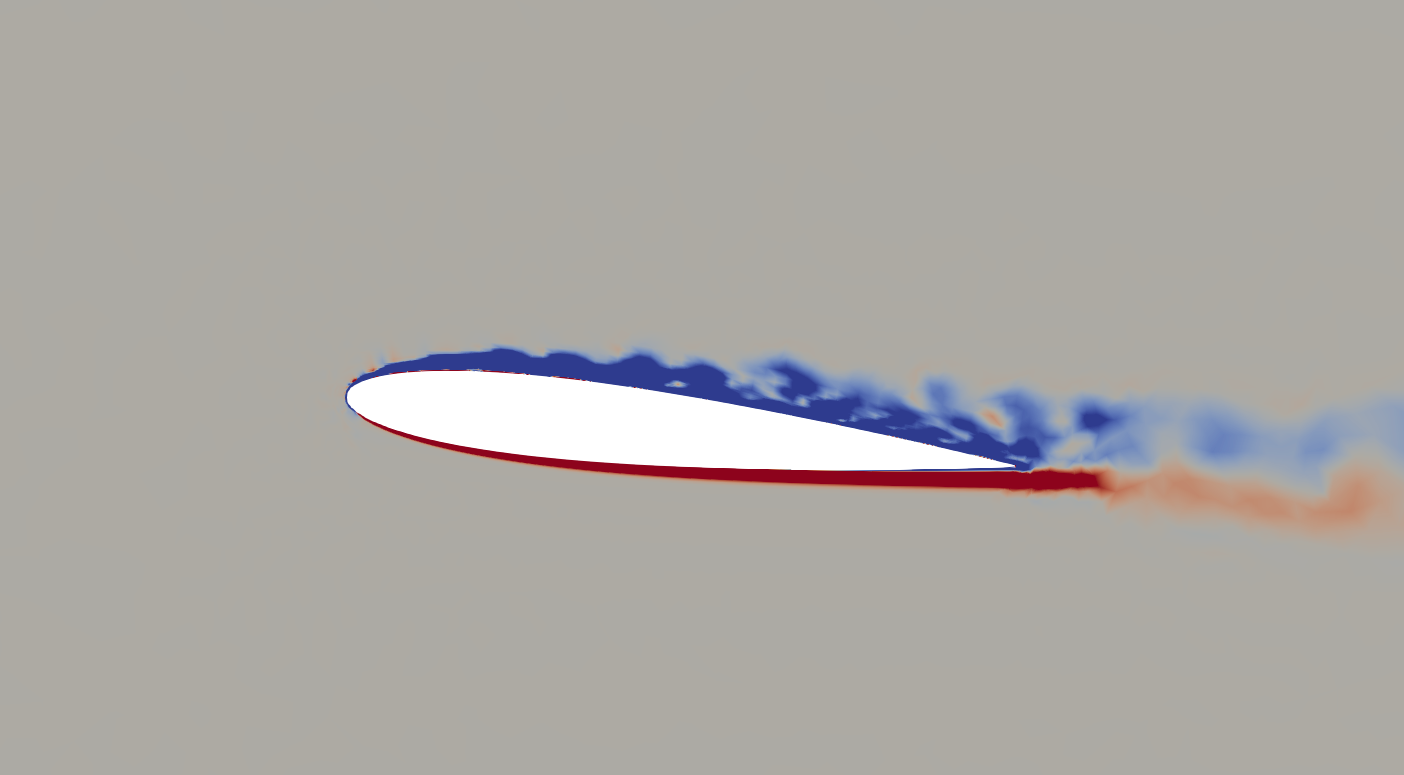
\includegraphics[width=1\textwidth]{figures/adapt_strat/vorticity_plots/M0/phase_195.png}
\caption{M0\_nz25 mesh at $\psi$ = $195^\circ$}
\label{fig:M0_psi195}
\end{subfigure}
\begin{subfigure}[b]{0.475\textwidth}
\centering
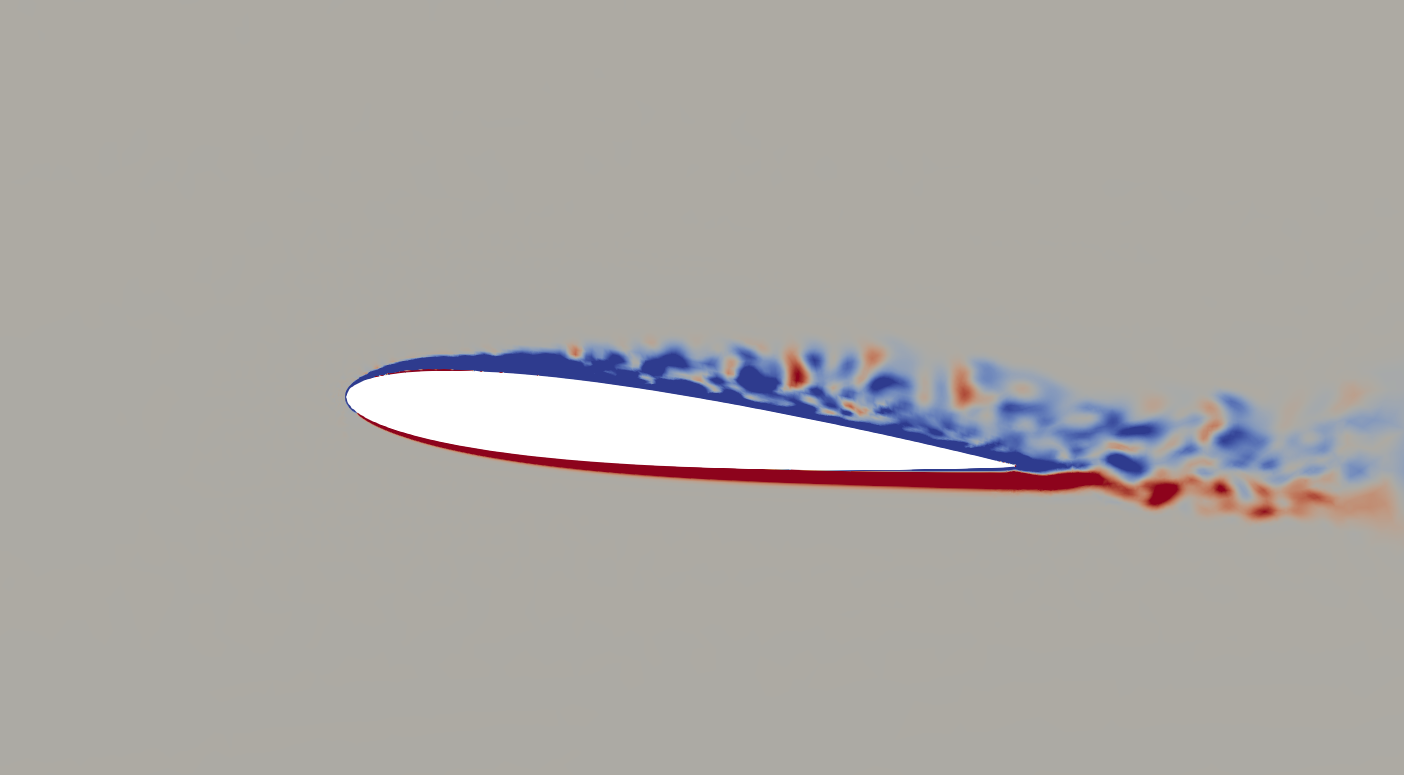
\includegraphics[width=1\textwidth]{figures/adapt_strat/vorticity_plots/Mza1_50/phase_195.png}
\caption{Mza1\_nz50 mesh at $\psi$ = $195^\circ$}
\label{fig:Ma1_psi195}
\end{subfigure}
%\begin{subfigure}[b]{0.475\textwidth}
%\centering
%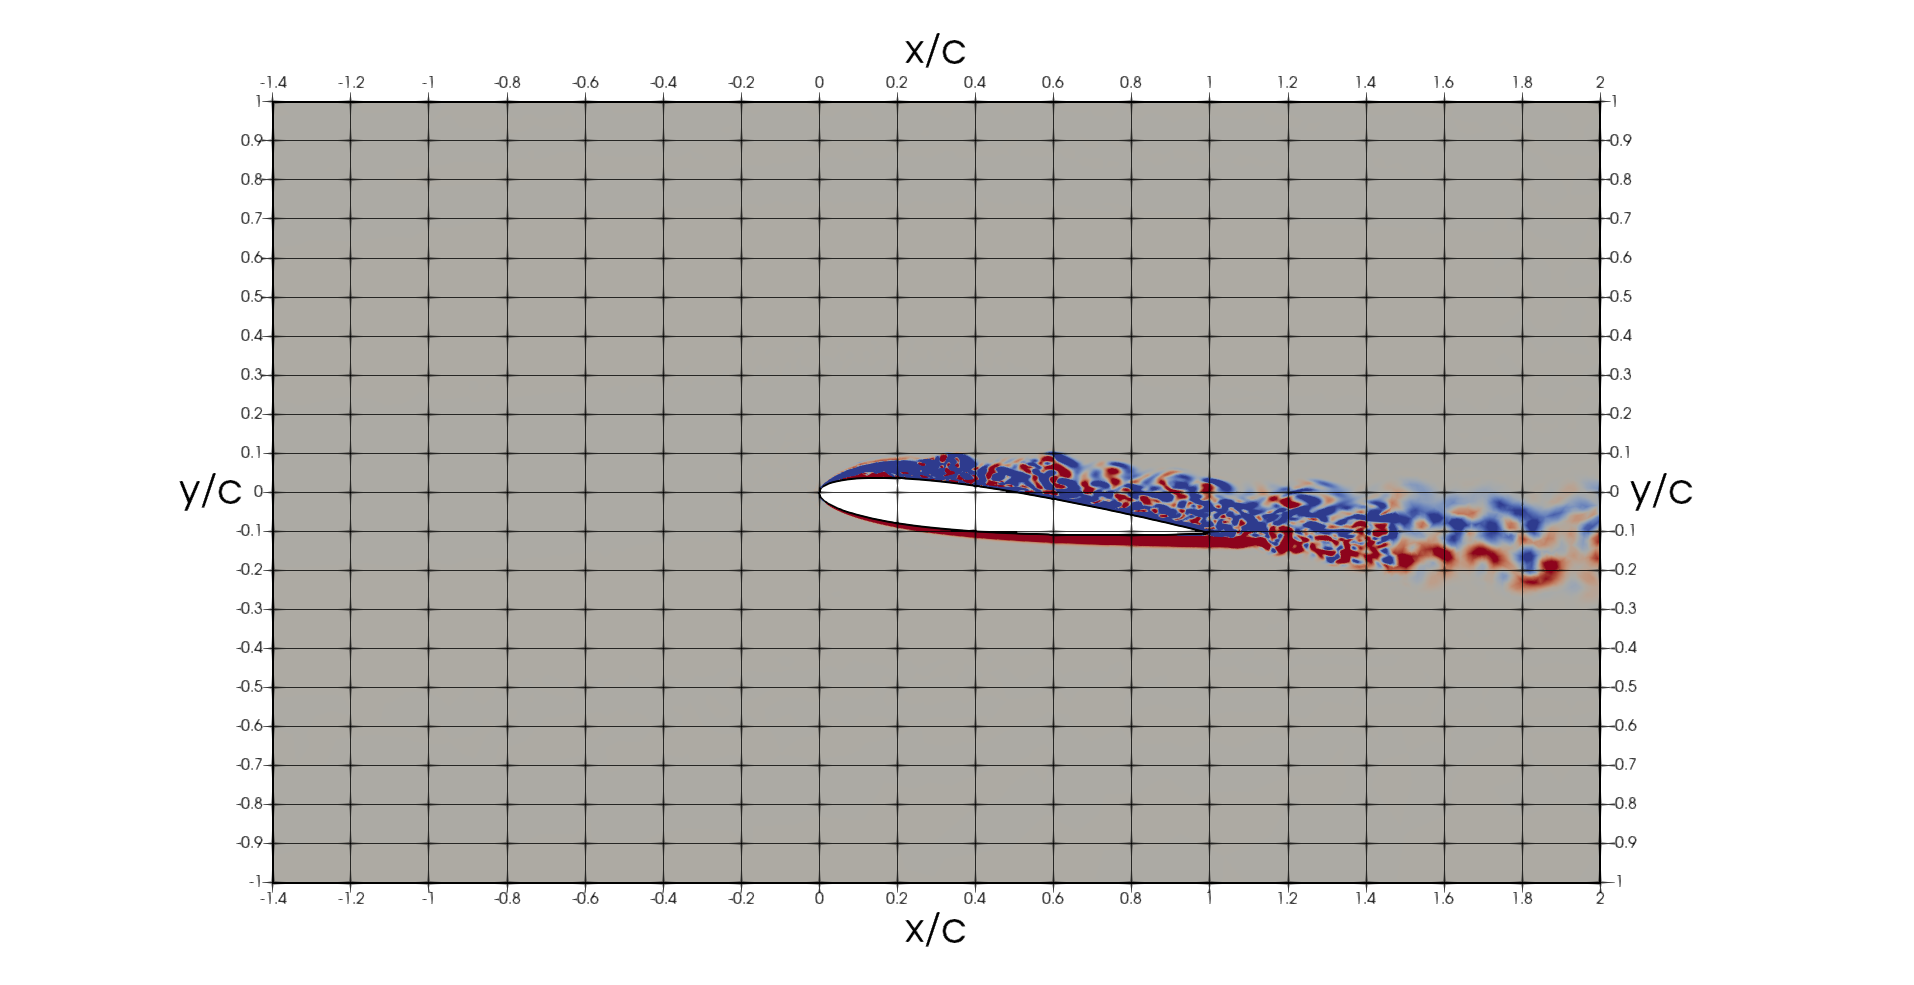
\includegraphics[width=1.25\textwidth]{figures/vorticity_plots/Mza2/ph_195.png}
%\caption{Mz\_a2 mesh, $\psi$ = $195^\circ$}
%\label{fig:Ma2_psi195}
%\end{subfigure}
\begin{subfigure}[b]{0.475\textwidth}
\centering
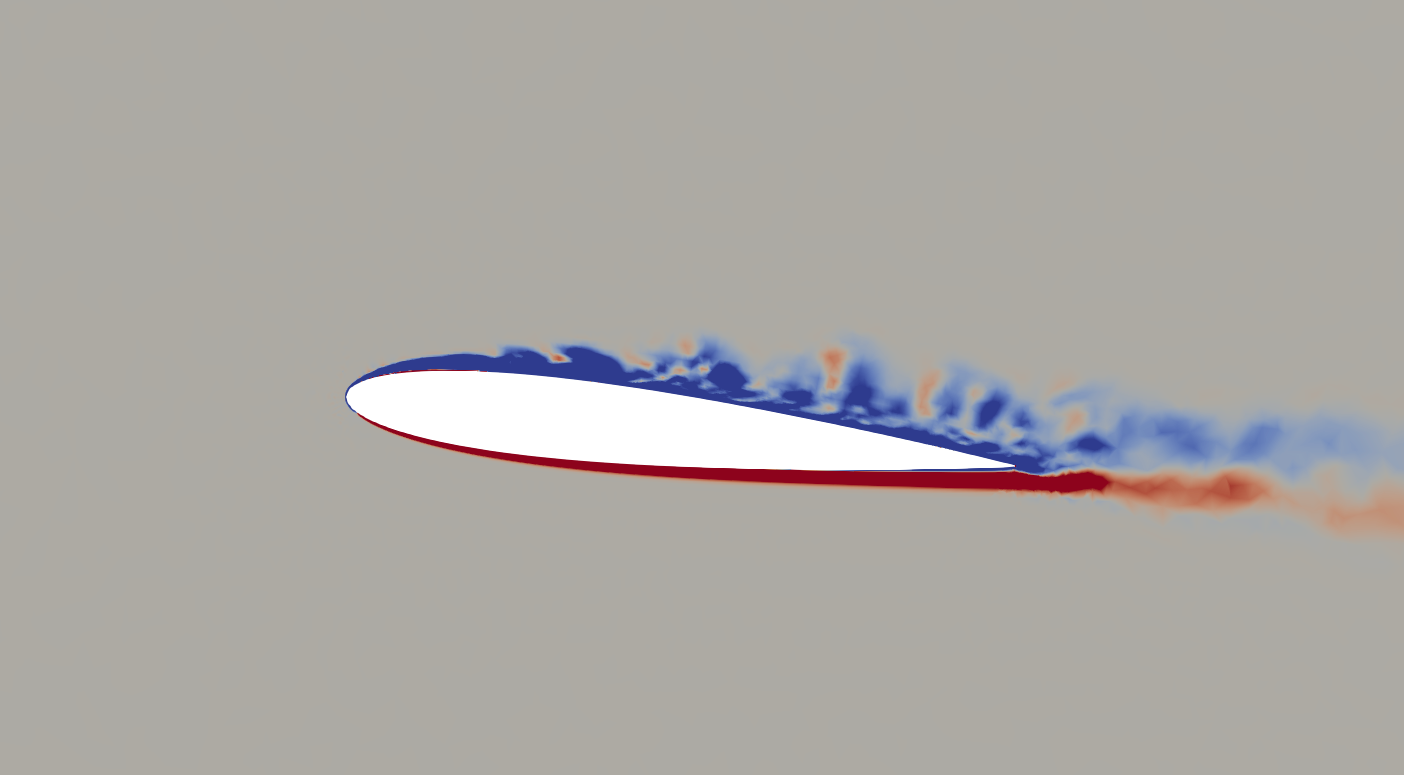
\includegraphics[width=1\textwidth]{figures/adapt_strat/vorticity_plots/Msa1_50/phase_195.png}
\caption{Msa1\_nz50 mesh at $\psi$ = $195^\circ$}
\label{fig:hadapt_psi195}
\end{subfigure}
\begin{subfigure}[b]{0.475\textwidth}
\centering
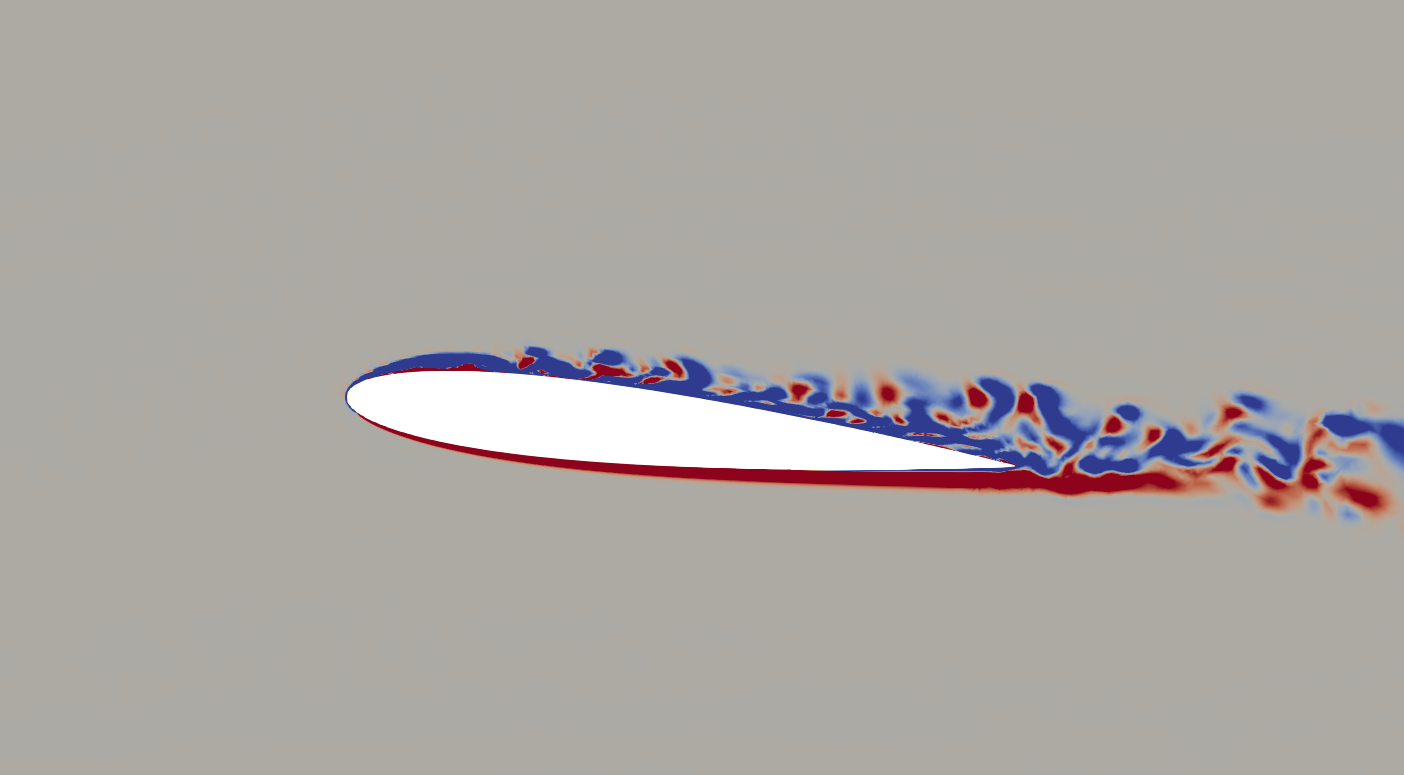
\includegraphics[width=1\textwidth]{figures/adapt_strat/vorticity_plots/Mfa1_50/phase_195.png}
\caption{Mfa1\_nz50 mesh at $\psi$ = $195^\circ$}
\label{fig:FB_psi195}
\end{subfigure}
\caption{Spanwise vorticity at $\psi$ = $195^\circ$ for different adaptive strategies/adapted meshes}
\label{fig:vorticity_195}
\end{figure}



\begin{figure}[H]
\centering
\begin{subfigure}[b]{0.475\textwidth}
\centering
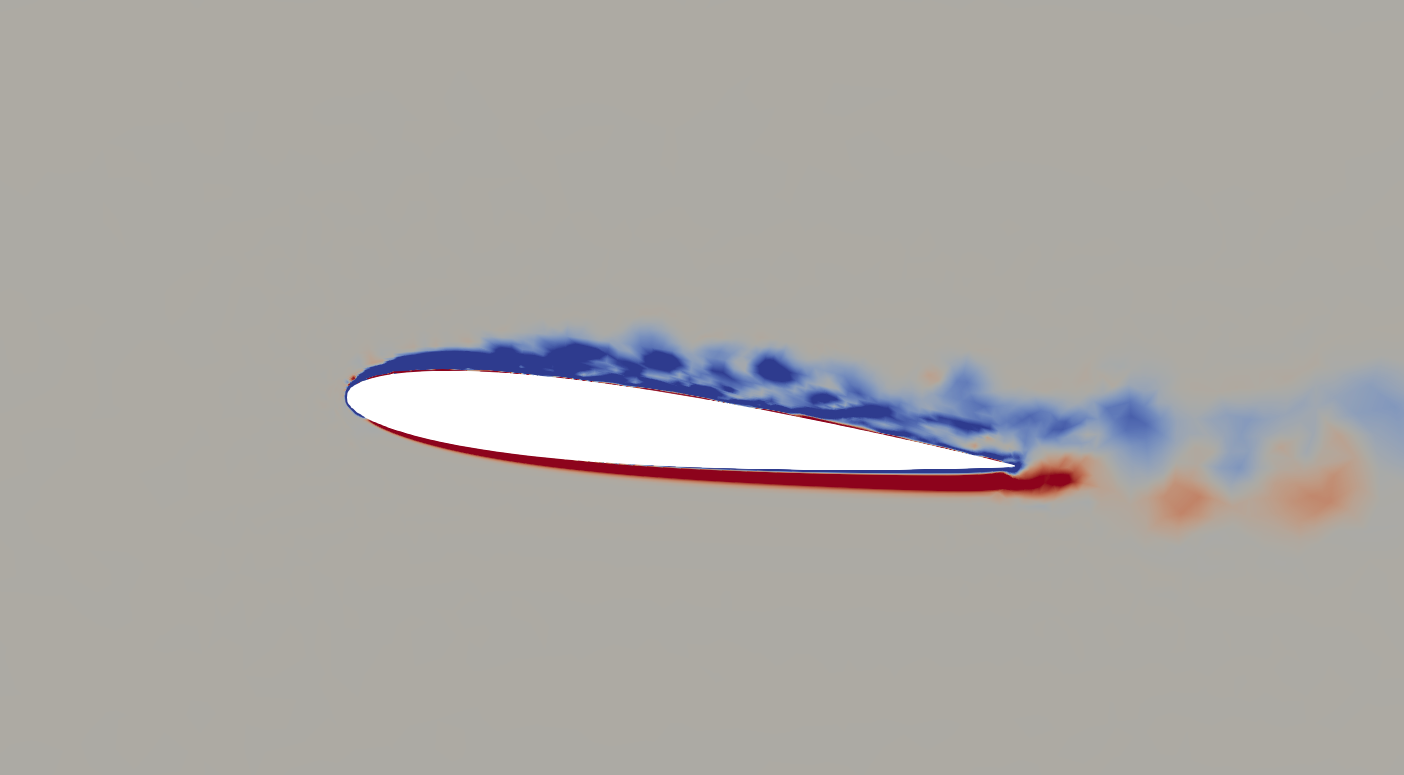
\includegraphics[width=1\textwidth]{figures/adapt_strat/vorticity_plots/M0/phase_210.png}
\caption{M0\_nz25 mesh at $\psi$ = $210^\circ$}
\label{fig:M0_psi210}
\end{subfigure}
\begin{subfigure}[b]{0.475\textwidth}
\centering
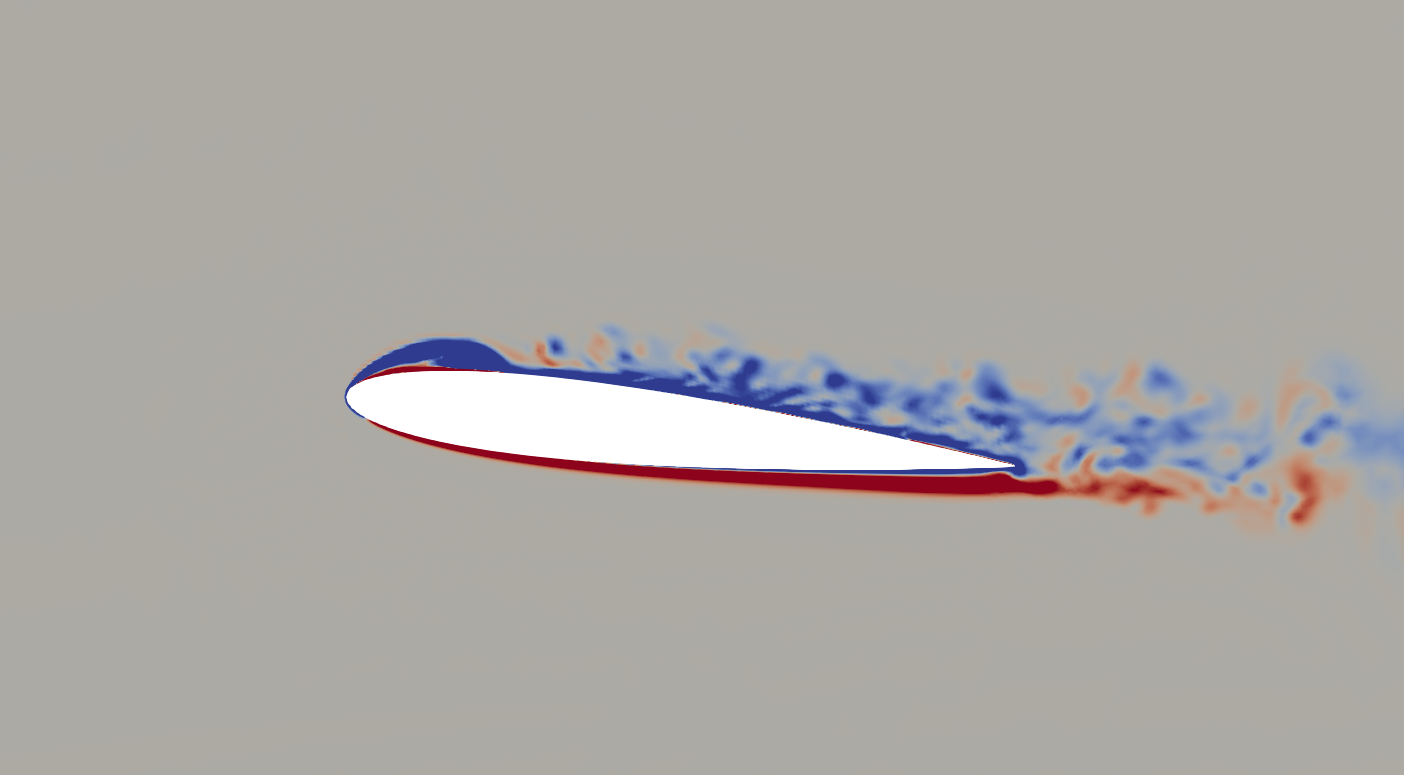
\includegraphics[width=1\textwidth]{figures/adapt_strat/vorticity_plots/Mza1_50/phase_210.png}
\caption{Mza1\_nz50 mesh at $\psi$ = $210^\circ$}
\label{fig:Mza1_psi210}
\end{subfigure}
%\begin{subfigure}[b]{0.475\textwidth}
%\centering
%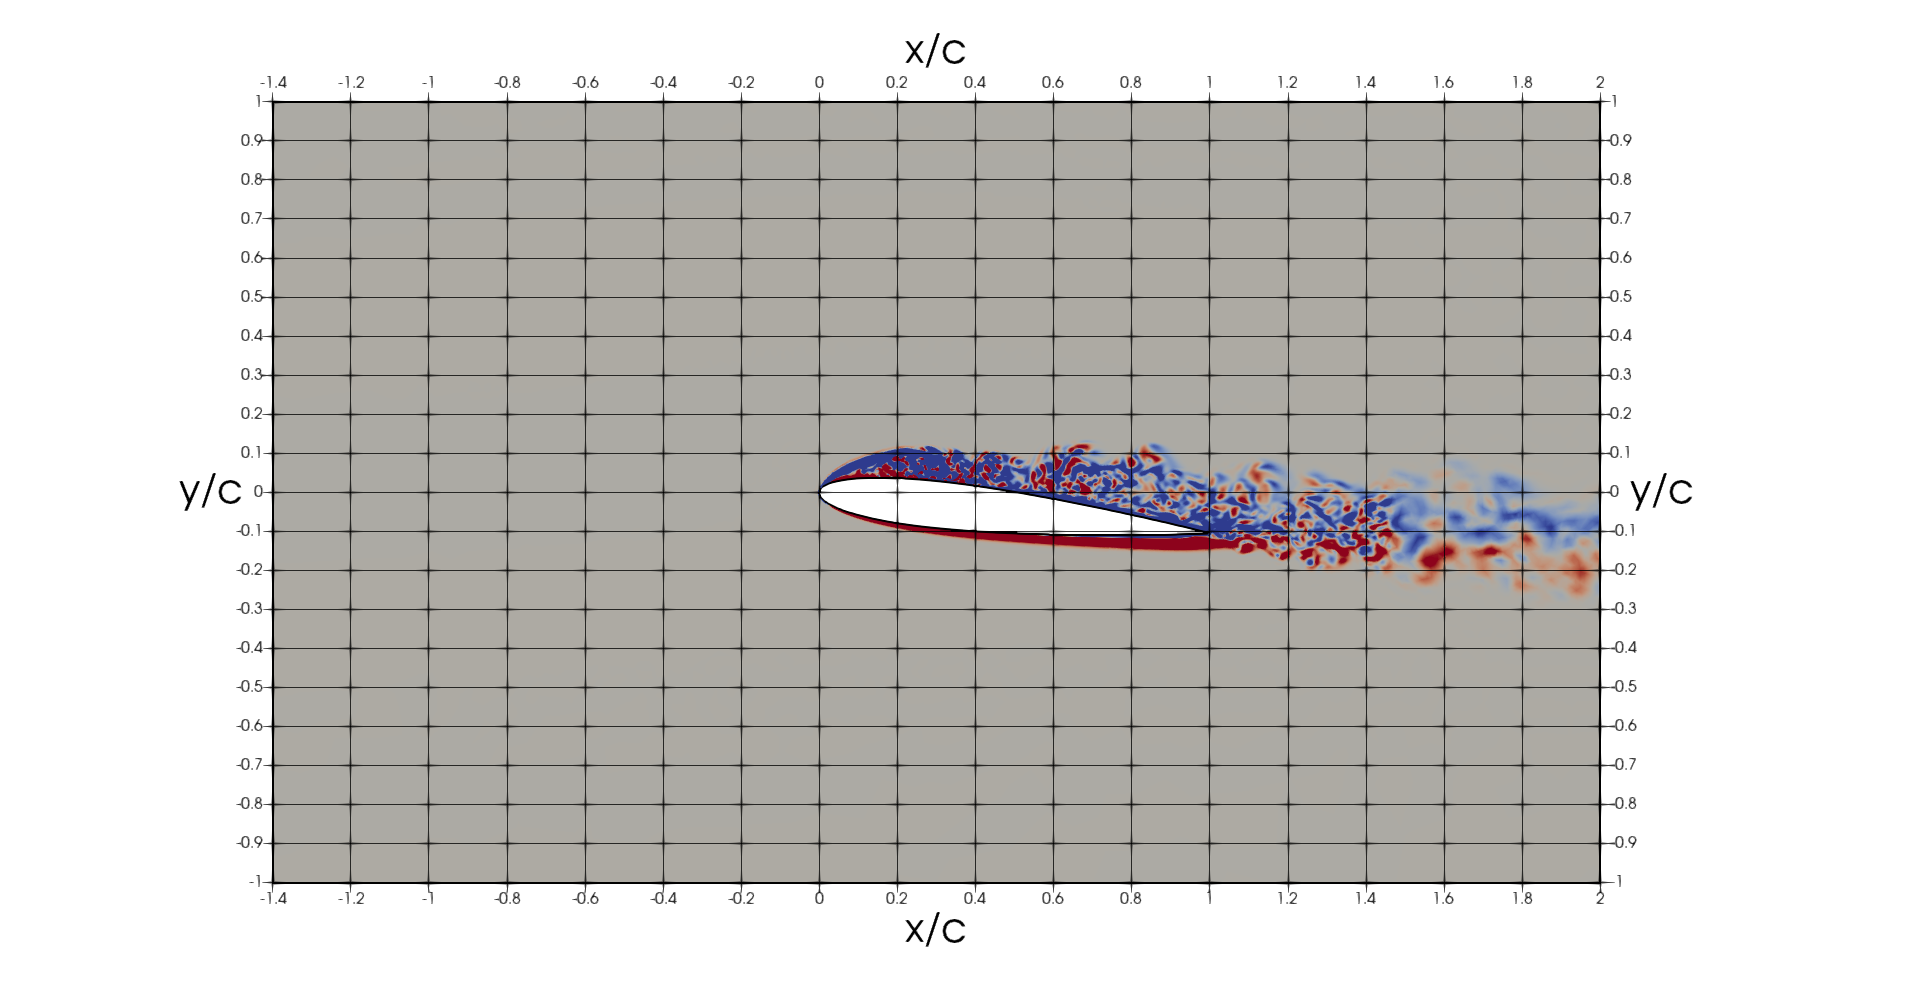
\includegraphics[width=1.25\textwidth]{figures/vorticity_plots/Mza2/ph_210.png}
%\caption{Mz\_a2 mesh, $\psi$ = $210^\circ$}
%\label{fig:Ma2_psi210}
%\end{subfigure}
\begin{subfigure}[b]{0.475\textwidth}
\centering
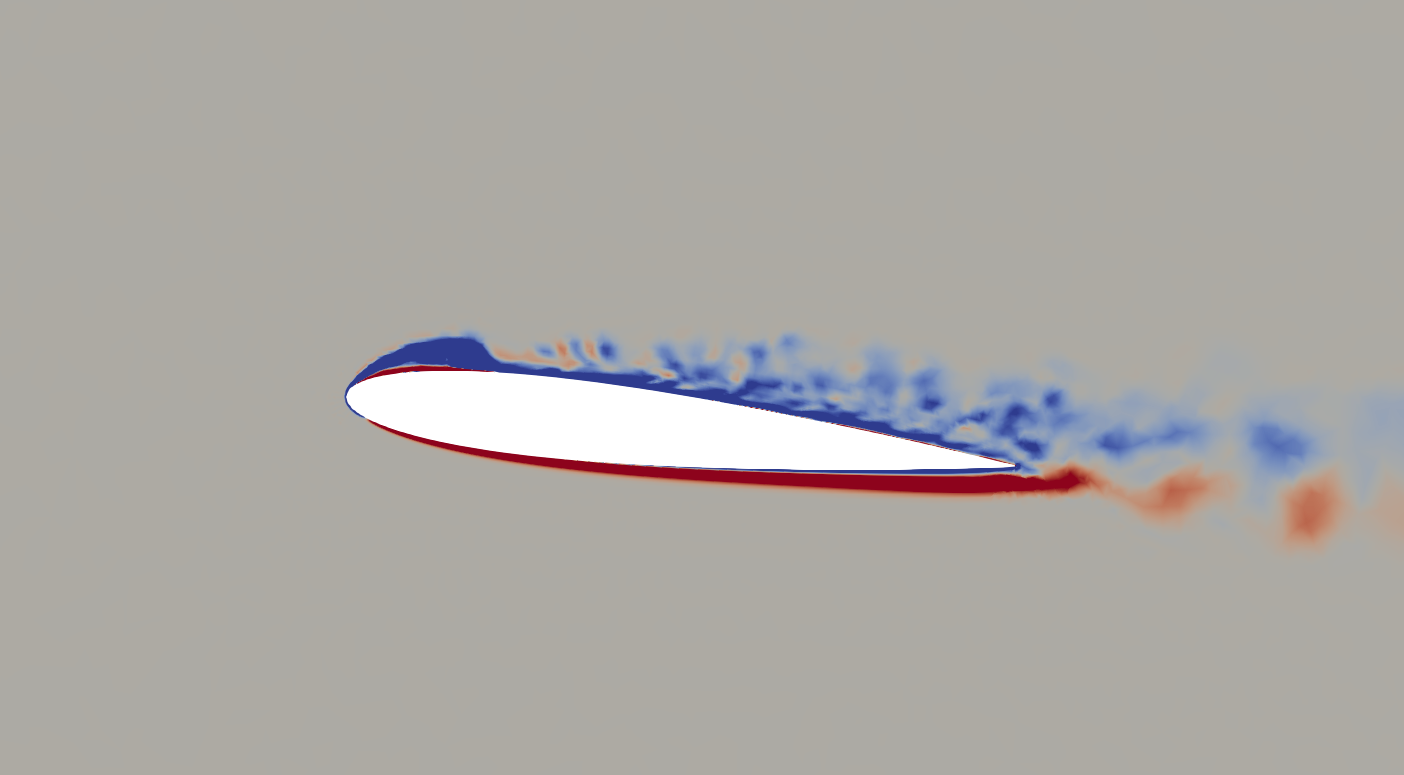
\includegraphics[width=1\textwidth]{figures/adapt_strat/vorticity_plots/Msa1_50/phase_210.png}
\caption{Msa1\_nz50 mesh at $\psi$ = $210^\circ$}
\label{fig:hadapt_psi210}
\end{subfigure}
\begin{subfigure}[b]{0.475\textwidth}
\centering
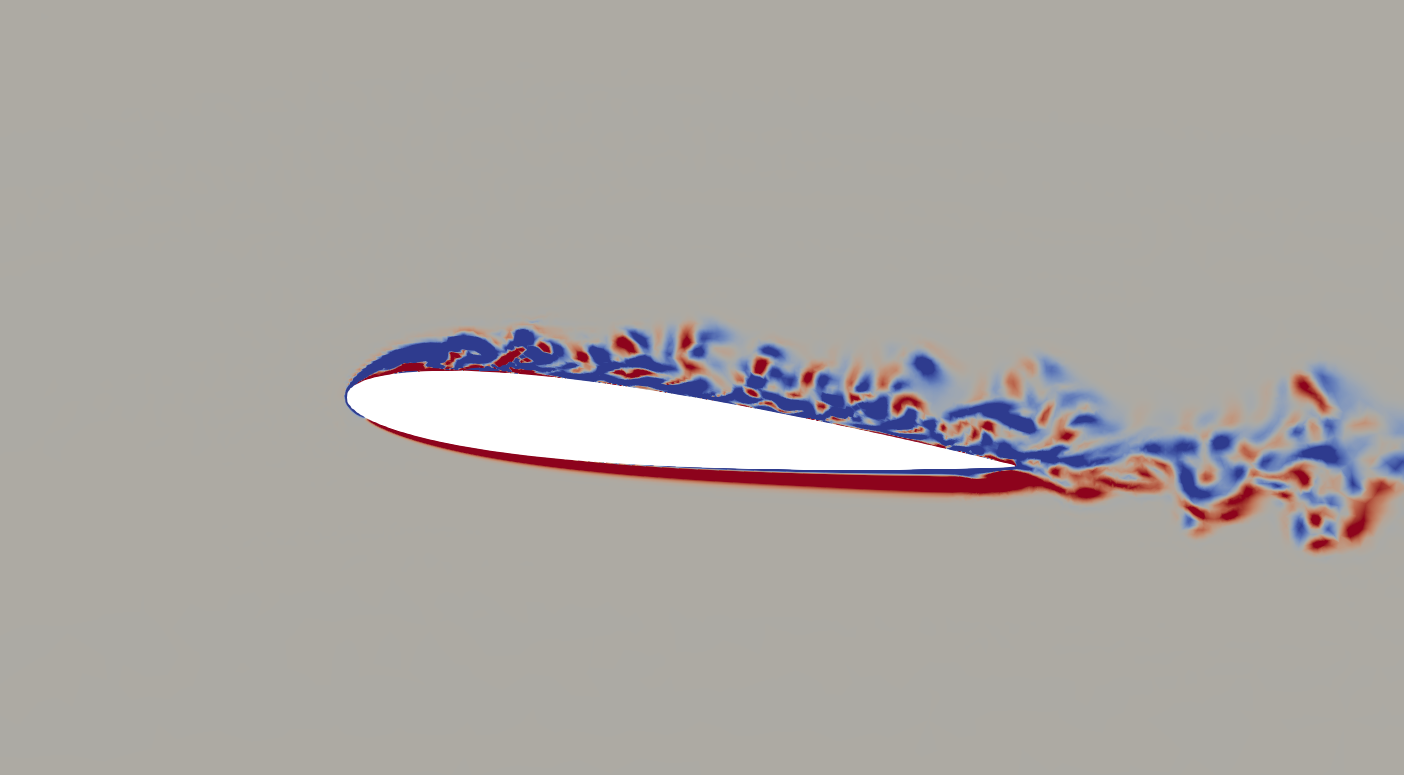
\includegraphics[width=1\textwidth]{figures/adapt_strat/vorticity_plots/Mfa1_50/phase_210.png}
\caption{Mfa1\_nz50 mesh at $\psi$ = $210^\circ$}
\label{fig:FB_psi210}
\end{subfigure}
\caption{Spanwise vorticity at $\psi$ = $210^\circ$ for different adaptive strategies/adapted meshes}
\label{fig:vorticity_210}
\end{figure}



%%VORTICITY PLOT
\begin{figure}[H]
\centering

\begin{subfigure}[b]{0.475\textwidth}
\centering
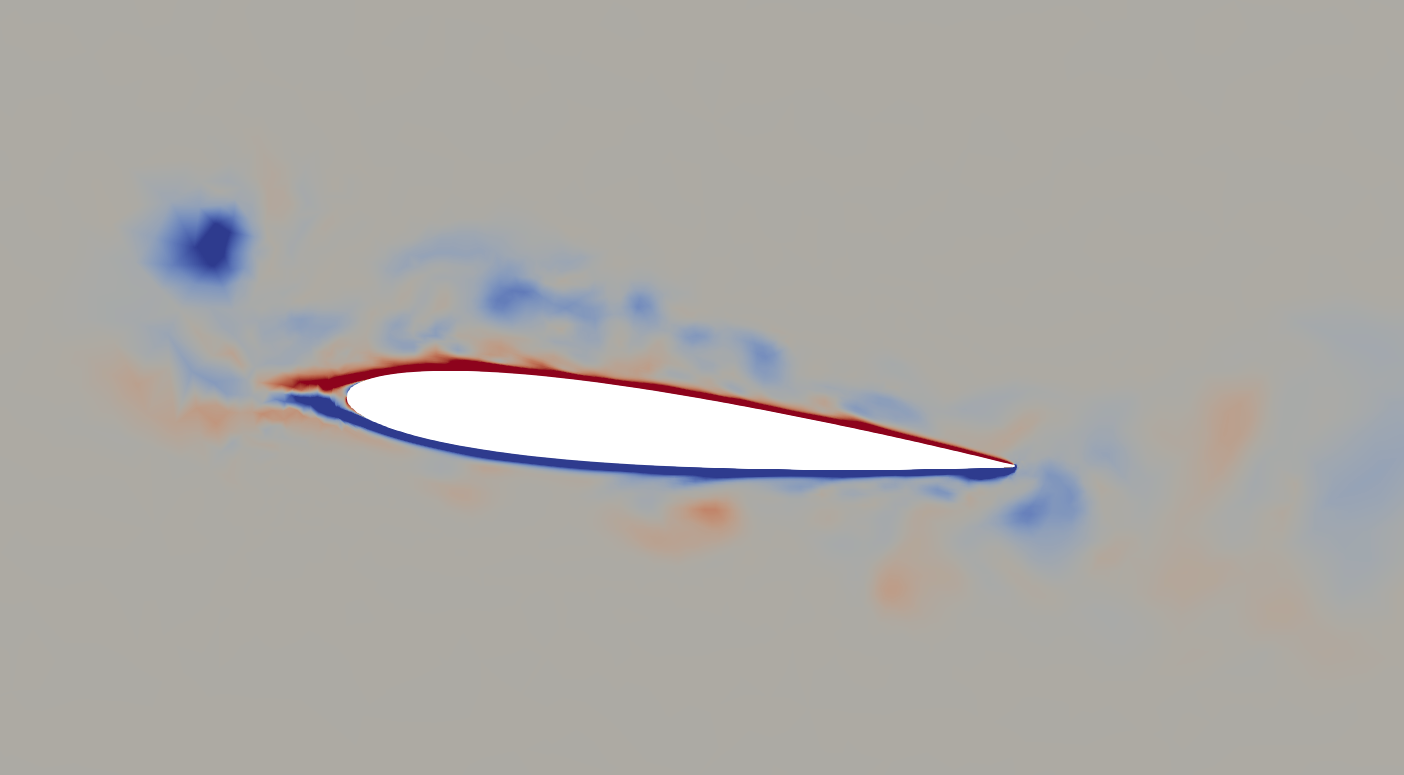
\includegraphics[width=1\textwidth]{figures/adapt_strat/vorticity_plots/M0/phase_270.png}
\caption{M0\_nz25 mesh at $\psi$ = $270^\circ$}
\label{fig:M0_psi270}
\end{subfigure}
\begin{subfigure}[b]{0.475\textwidth}
\centering
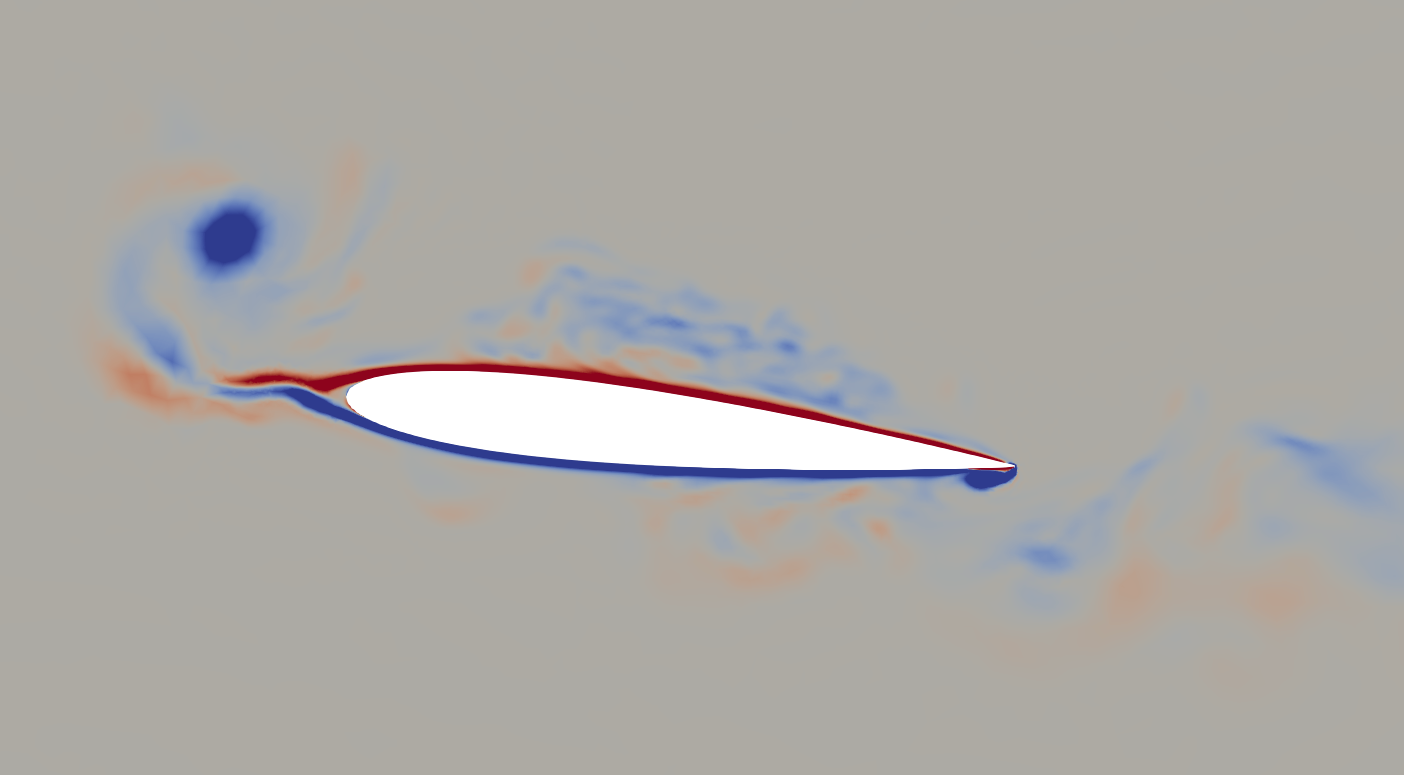
\includegraphics[width=1\textwidth]{figures/adapt_strat/vorticity_plots/Mza1_50/phase_270.png}
\caption{Mza1\_nz50 mesh at $\psi$ = $270^\circ$}
\label{fig:Ma1_psi270}
\end{subfigure}
%\begin{subfigure}[b]{0.475\textwidth}
%\centering
%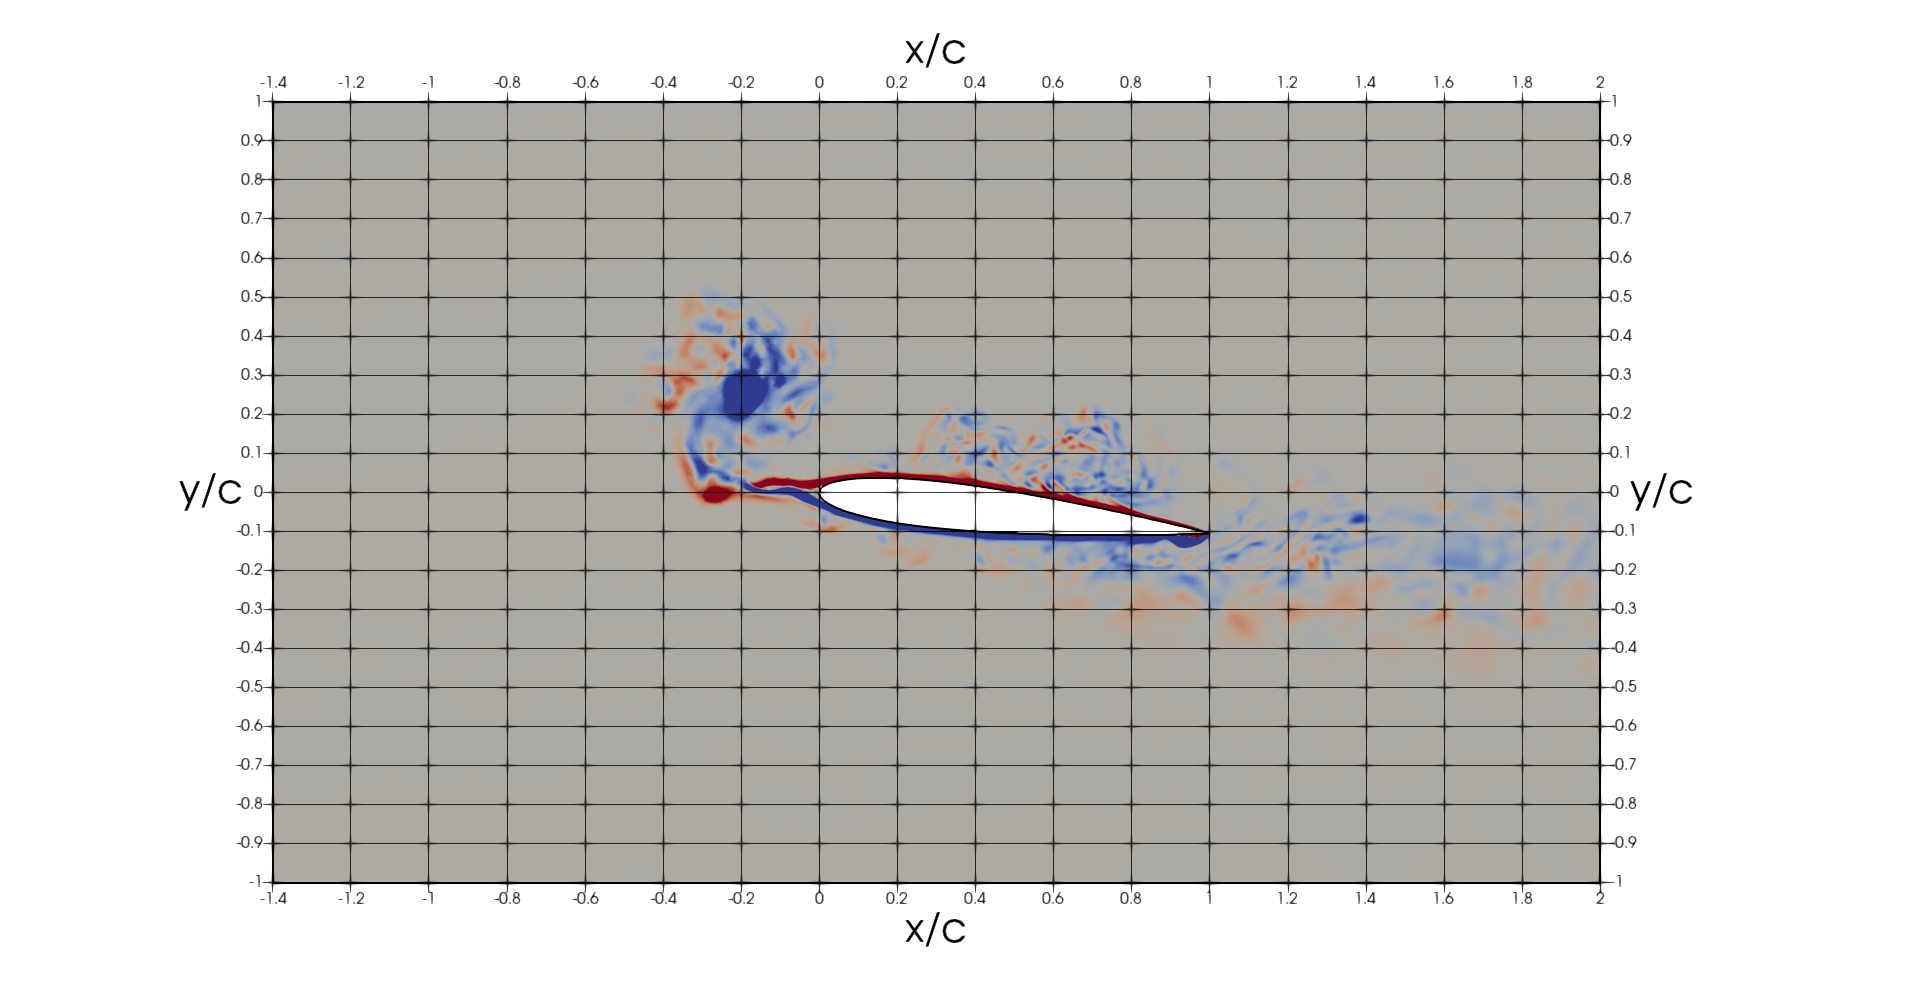
\includegraphics[width=1.25\textwidth]{figures/vorticity_plots/Mza2/ph_270.png}
%\caption{Mz\_a2 mesh, $\psi$ = $270^\circ$}
%\label{fig:Ma2_psi270}
%\end{subfigure}
\begin{subfigure}[b]{0.475\textwidth}
\centering
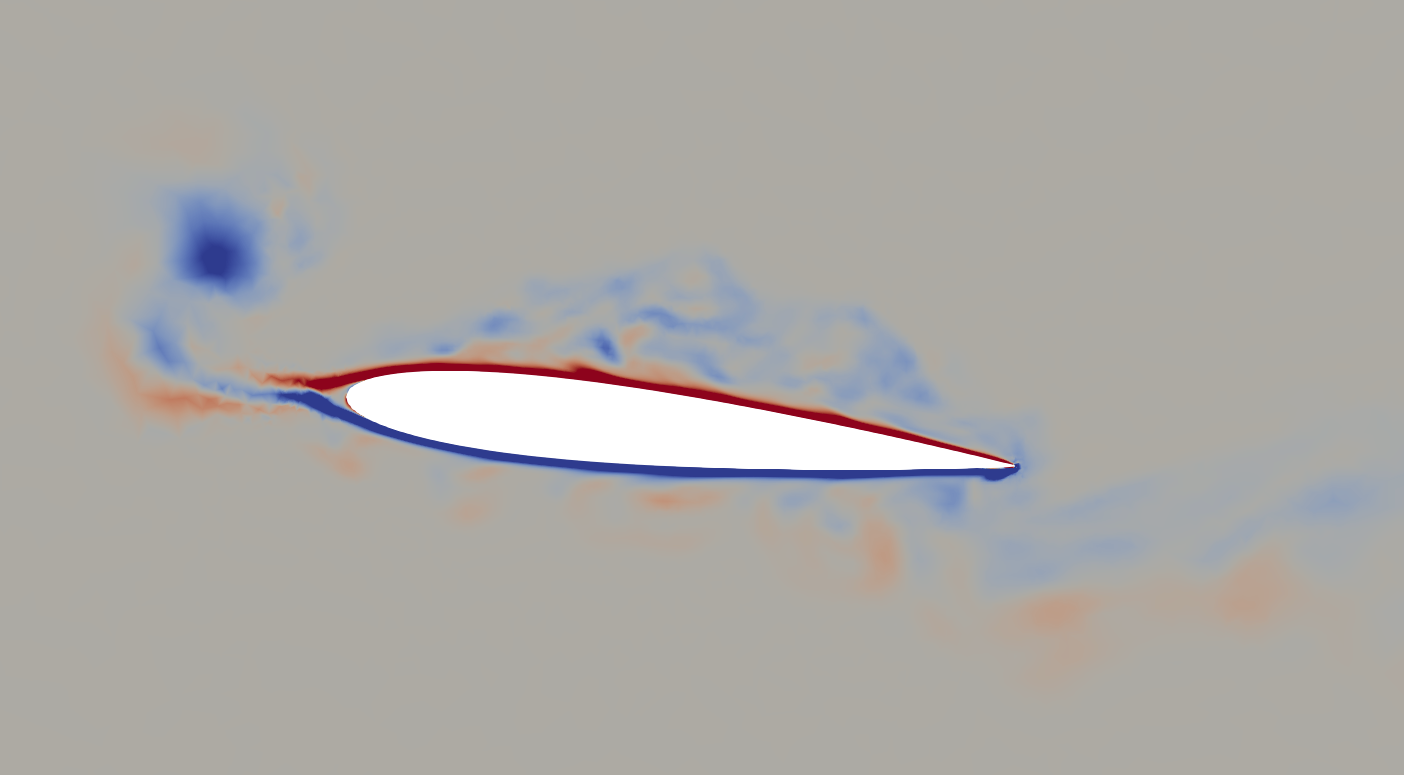
\includegraphics[width=1\textwidth]{figures/adapt_strat/vorticity_plots/Msa1_50/phase_270.png}
\caption{Msa1\_nz50 mesh at $\psi$ = $270^\circ$}
\label{fig:hadapt_psi270}
\end{subfigure}
\begin{subfigure}[b]{0.475\textwidth}
\centering
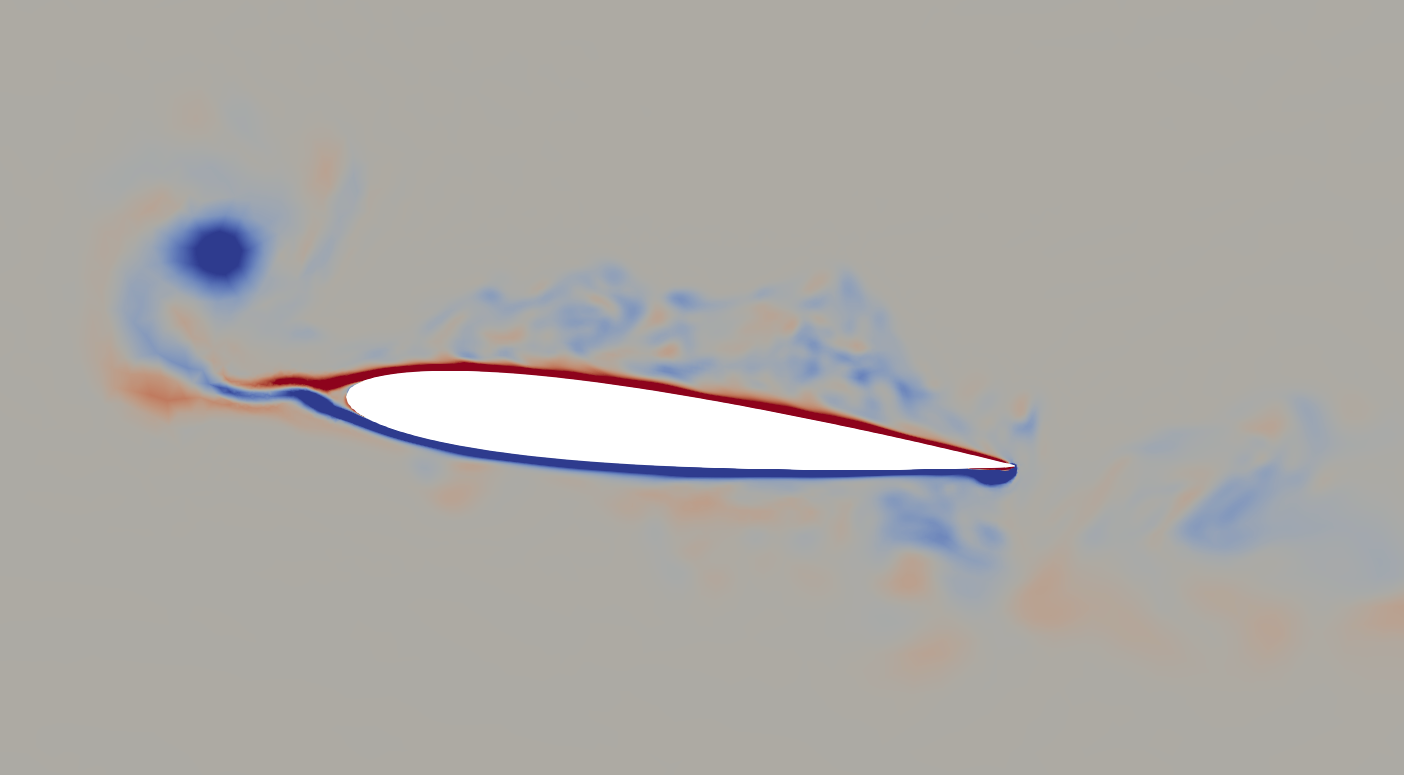
\includegraphics[width=1\textwidth]{figures/adapt_strat/vorticity_plots/Mfa1_50/phase_270.png}
\caption{Mfa1\_nz50 mesh at $\psi$ = $270^\circ$}
\label{fig:FB_psi270}
\end{subfigure}
\caption{Spanwise vorticity at $\psi$ = $270^\circ$ for different adaptive strategies/adapted meshes}
\label{fig:vorticity_270}
\end{figure}

Figures \ref{fig:Mza1_zoomed}, \ref{fig:Msa1_zoomed} and \ref{fig:Mfa1_zoomed} show a zoomed-in view of the mesh, spanwise vorticity at $\psi=210^\circ$, and the element-level/local error (i.e., the maximum value over multiple phases and over the spanwise direction). This is done for Mza1\_nz50, Msa1\_nz50, and Mfa1\_nz50 meshes.
These figures show that a quasi-uniform mesh size is maintained in specified zones for both Mza1\_nz50 and Mfa1\_nz50, while the Msa1\_nz50 mesh is patchy, i.e., a uniform or quasi-uniform mesh size is not maintained in Msa1\_nz50 in crucial zones.
The error field for Msa1\_nz50 is also patchy, as compared to Mza1\_nz50 and Mfa1\_nz50, with elements that have a higher local estimated error in Msa1\_nz50.
This becomes further evident from the vorticity plots, especially in the wake region, where Msa1\_nz50 shows a poor resolution of the fine-scale flow structures as compared to Mza1\_nz50 and Mfa1\_nz50.
Note that the Mza1\_nz50 and Mfa1\_nz50 meshes are very comparable and the zonal refinement encompasses the regions/portions covered by the feature/LEV-based refinement, and thus, they turn out to be equivalent in their predictive capability for the current case.

\begin{figure}[H]
	\centering
\begin{subfigure}[b]{0.7\textwidth}
	\centering
	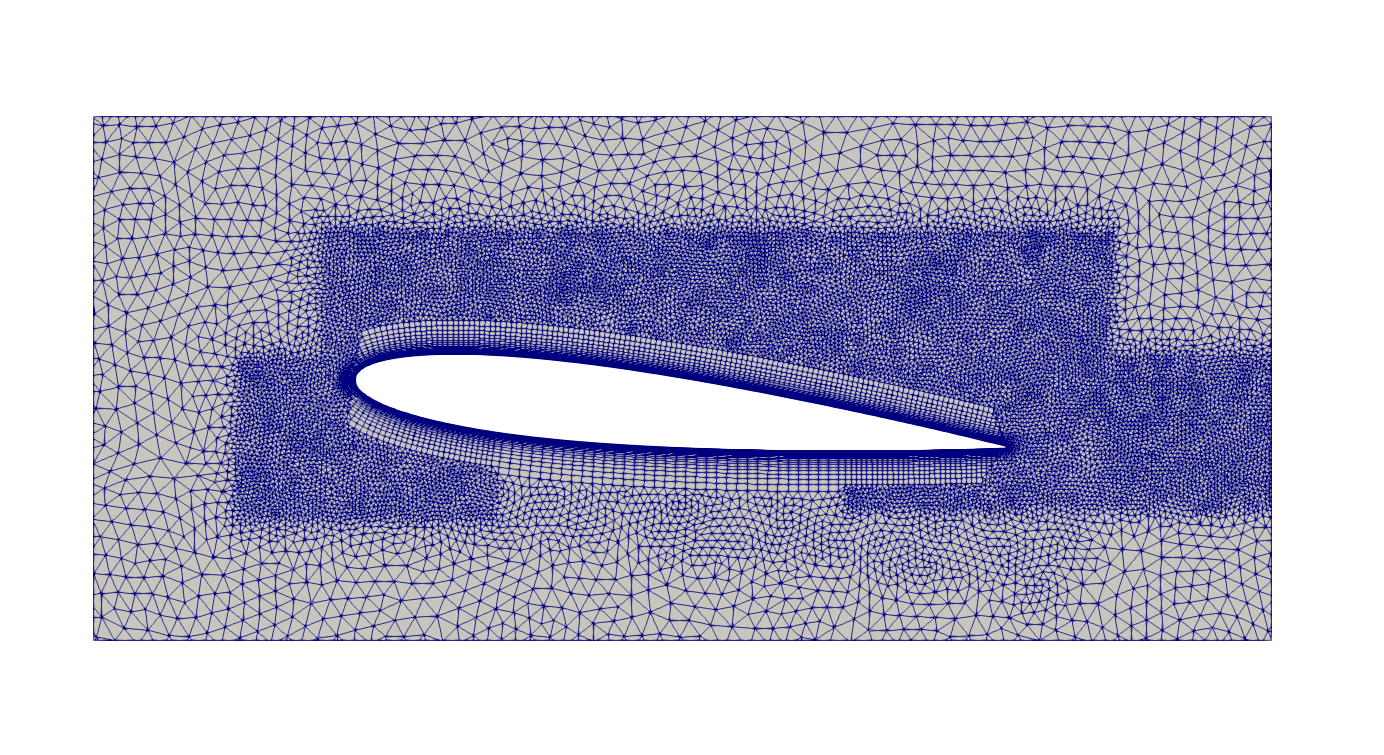
\includegraphics[width=1\textwidth]{figures/adapt_strat/zoomed/Mza1_mesh.png}
	\caption{Mza1\_nz50 mesh}
	\label{fig:Mza1_mesh_zoomed}
\end{subfigure}
\begin{subfigure}[b]{0.7\textwidth}
	\centering
	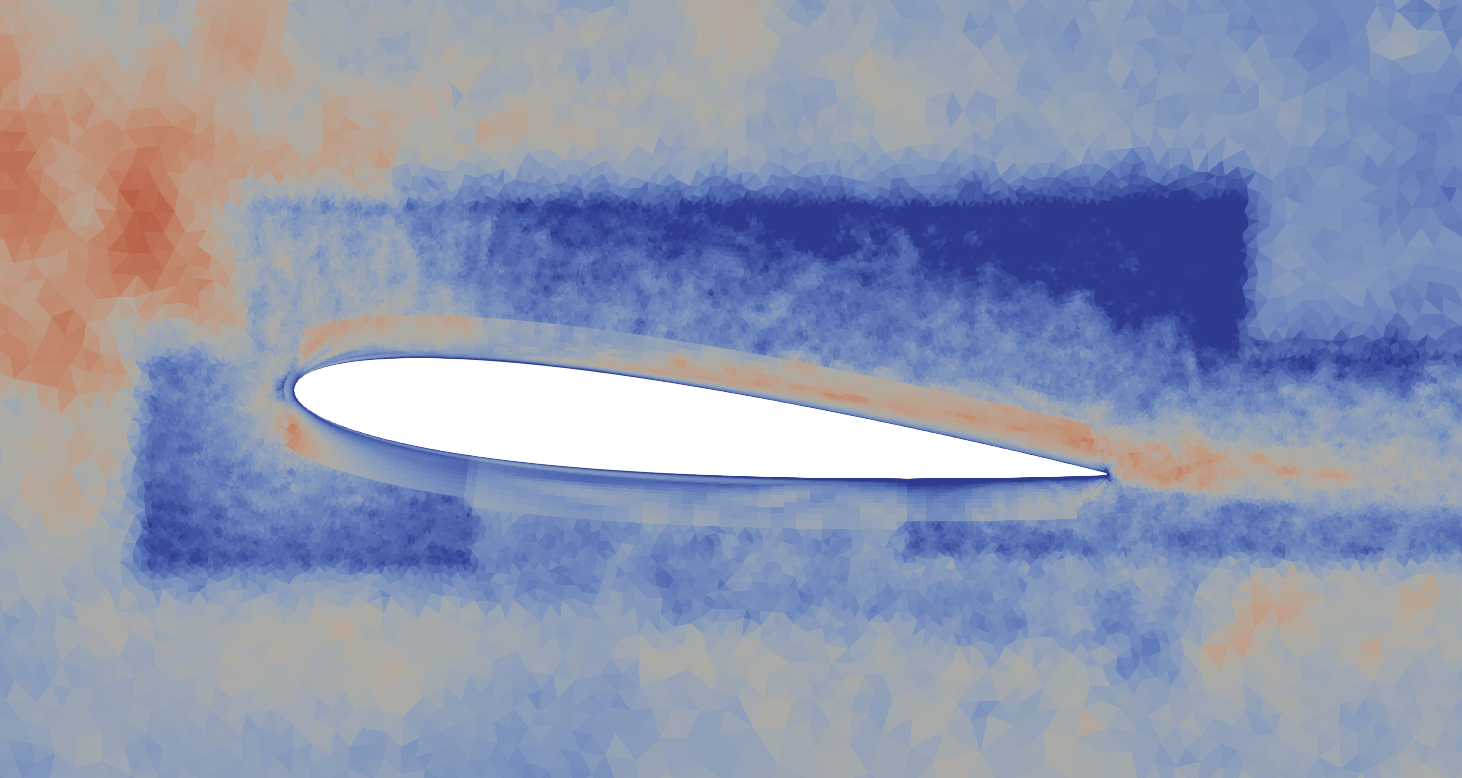
\includegraphics[width=1\textwidth]{figures/adapt_strat/zoomed/Mza1_error.png}
	\caption{Mza1\_nz50 estimated error}
	\label{fig:Mza1_max_error_zoomed}
\end{subfigure}
\begin{subfigure}[b]{0.7\textwidth}
	\centering
	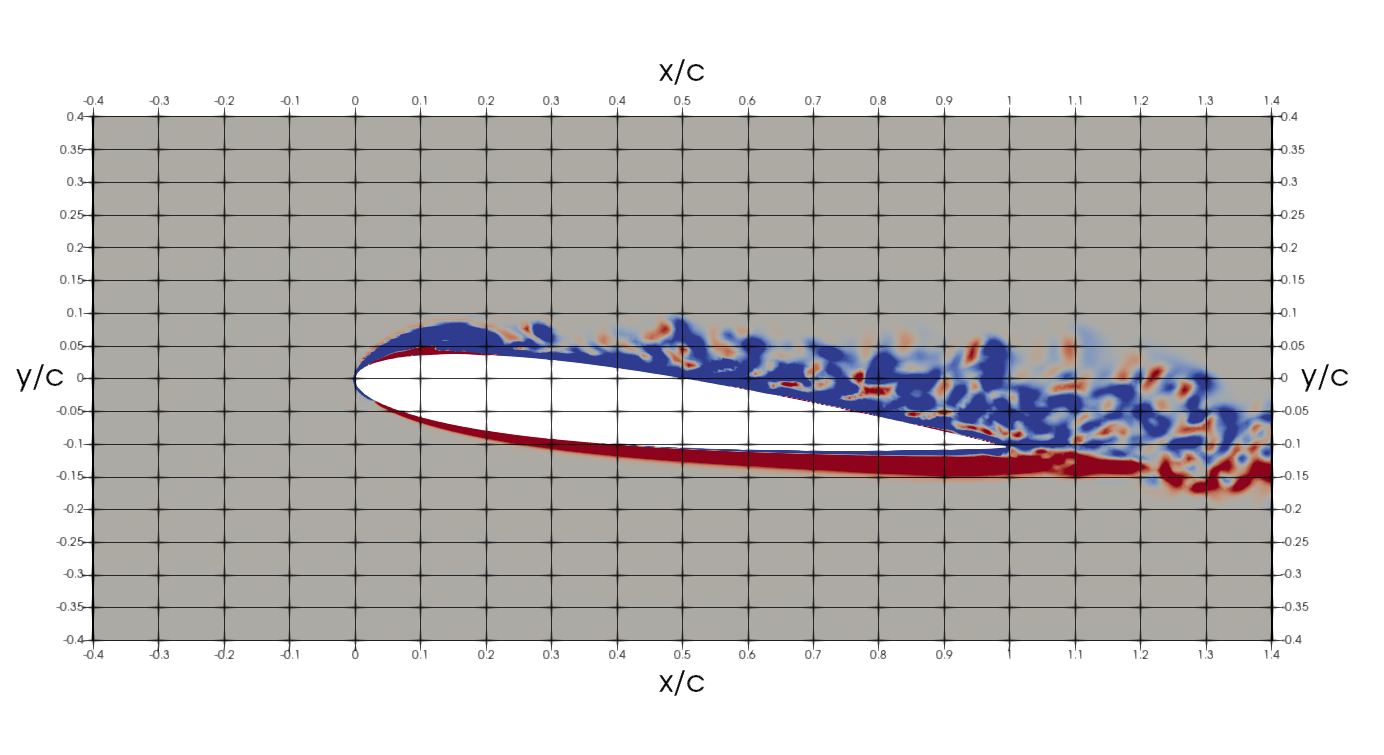
\includegraphics[width=1\textwidth]{figures/adapt_strat/zoomed/Mza1_ph_210.png}
	\caption{Mza1\_nz50 vorticity at $\psi=210^\circ$}
	\label{fig:Mza1_vorticity_zoomed}
\end{subfigure}
\caption{Zoomed-in view for Mza1\_nz50: mesh, estimated error and vorticity}
\label{fig:Mza1_zoomed}
\end{figure}

\begin{figure}[H]
	\centering
	\begin{subfigure}[b]{0.7\textwidth}
		\centering
		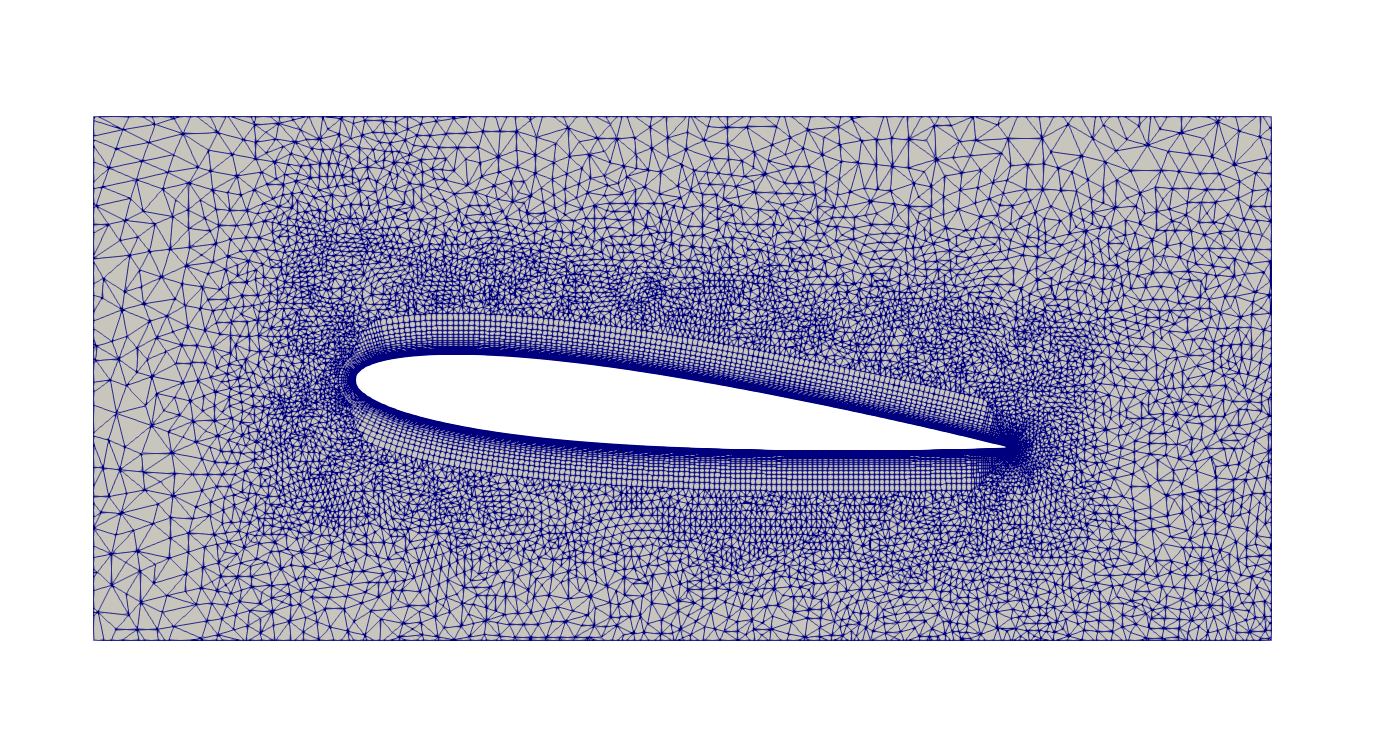
\includegraphics[width=1\textwidth]{figures/adapt_strat/zoomed/Msa1_mesh.png}
		\caption{Msa1\_nz50 mesh}
		\label{fig:Msa1_mesh_zoomed}
	\end{subfigure}
	\begin{subfigure}[b]{0.7\textwidth}
		\centering
		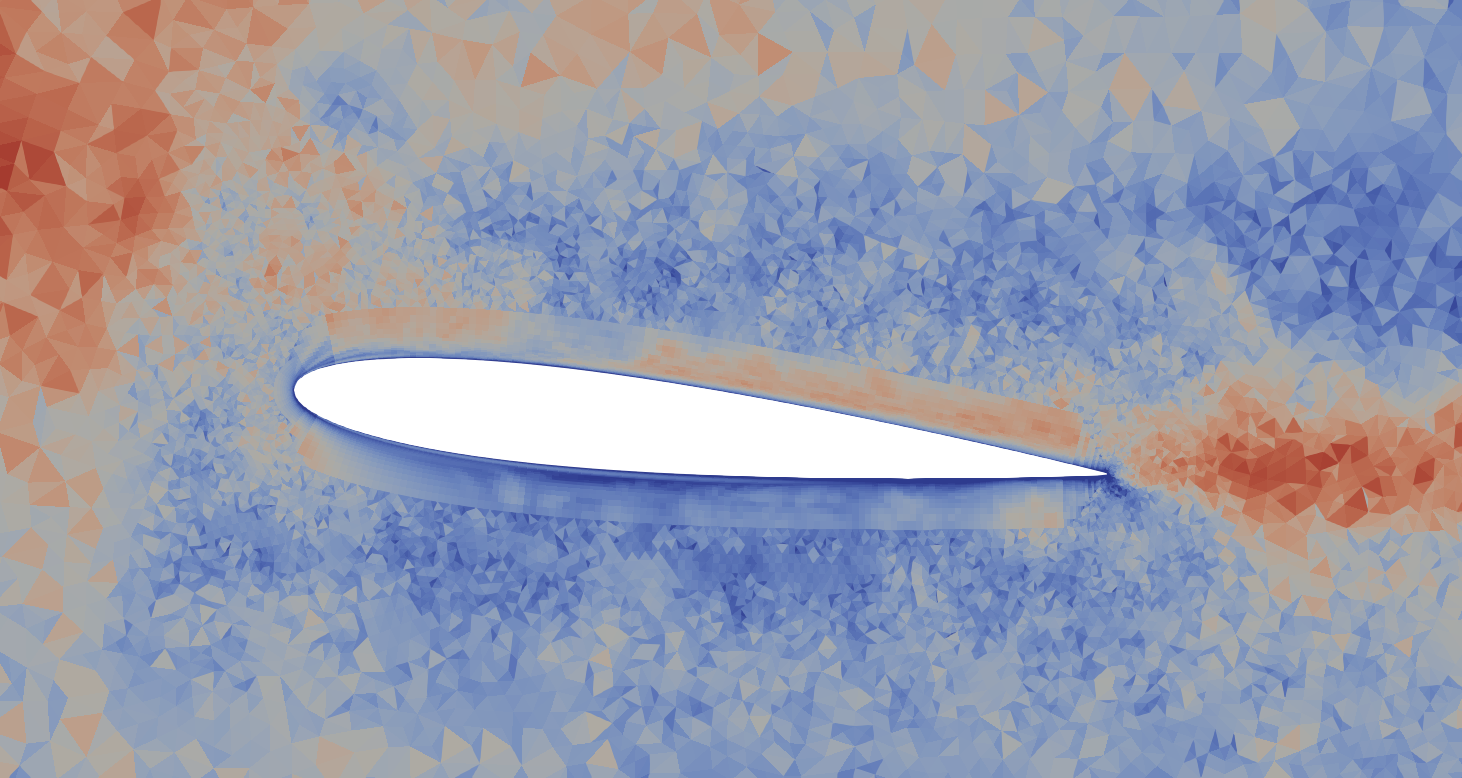
\includegraphics[width=1\textwidth]{figures/adapt_strat/zoomed/Msa1_error.png}
		\caption{Msa1\_nz50 estimated error}
		\label{fig:Msa1_max_error_zoomed}
	\end{subfigure}
	\begin{subfigure}[b]{0.7\textwidth}
		\centering
		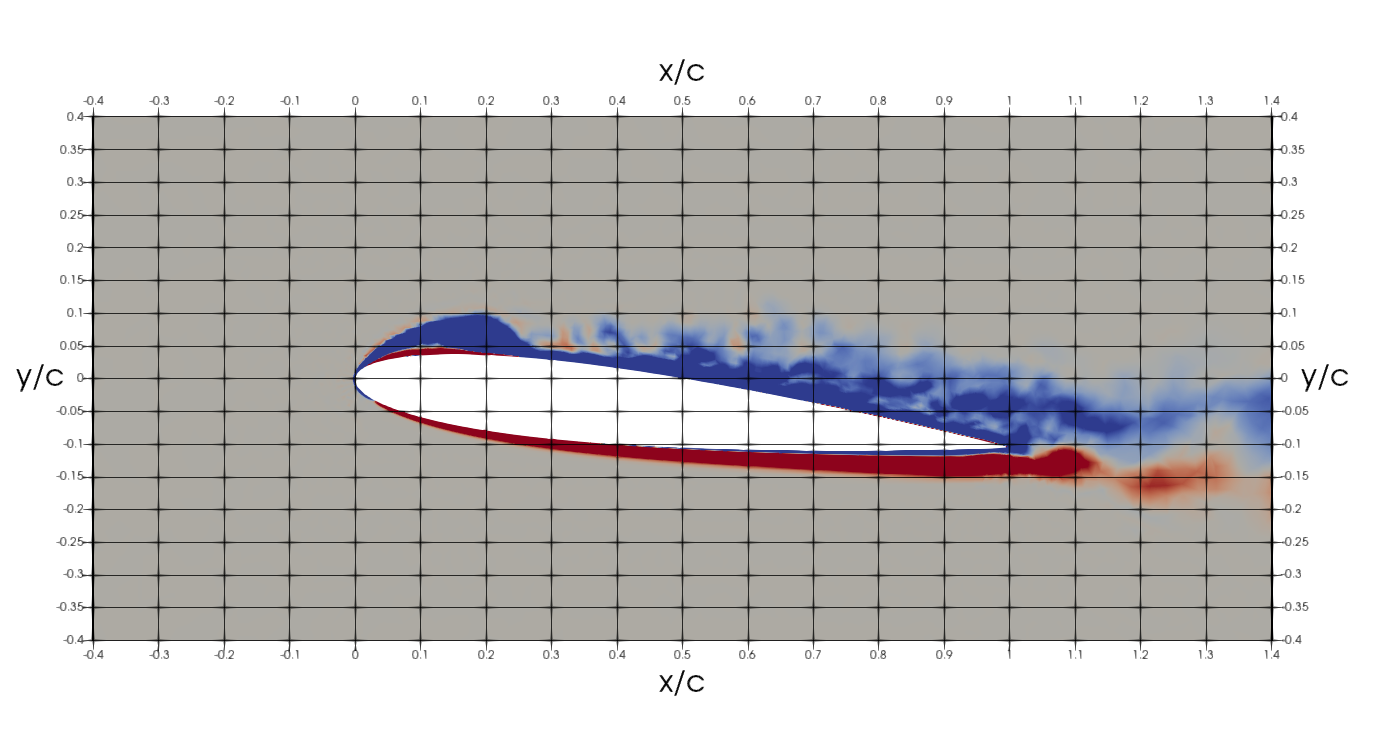
\includegraphics[width=1\textwidth]{figures/adapt_strat/zoomed/Msa1_ph_210.png}
		\caption{Msa1\_nz50 vorticity at $\psi=210^\circ$}
		\label{fig:Msa1_vorticity_zoomed}
	\end{subfigure}
	\caption{Zoomed-in view for Msa1\_nz50: mesh, estimated error and vorticity}
	\label{fig:Msa1_zoomed}
\end{figure}


\begin{figure}[H]
	\centering
	\begin{subfigure}[b]{0.7\textwidth}
		\centering
		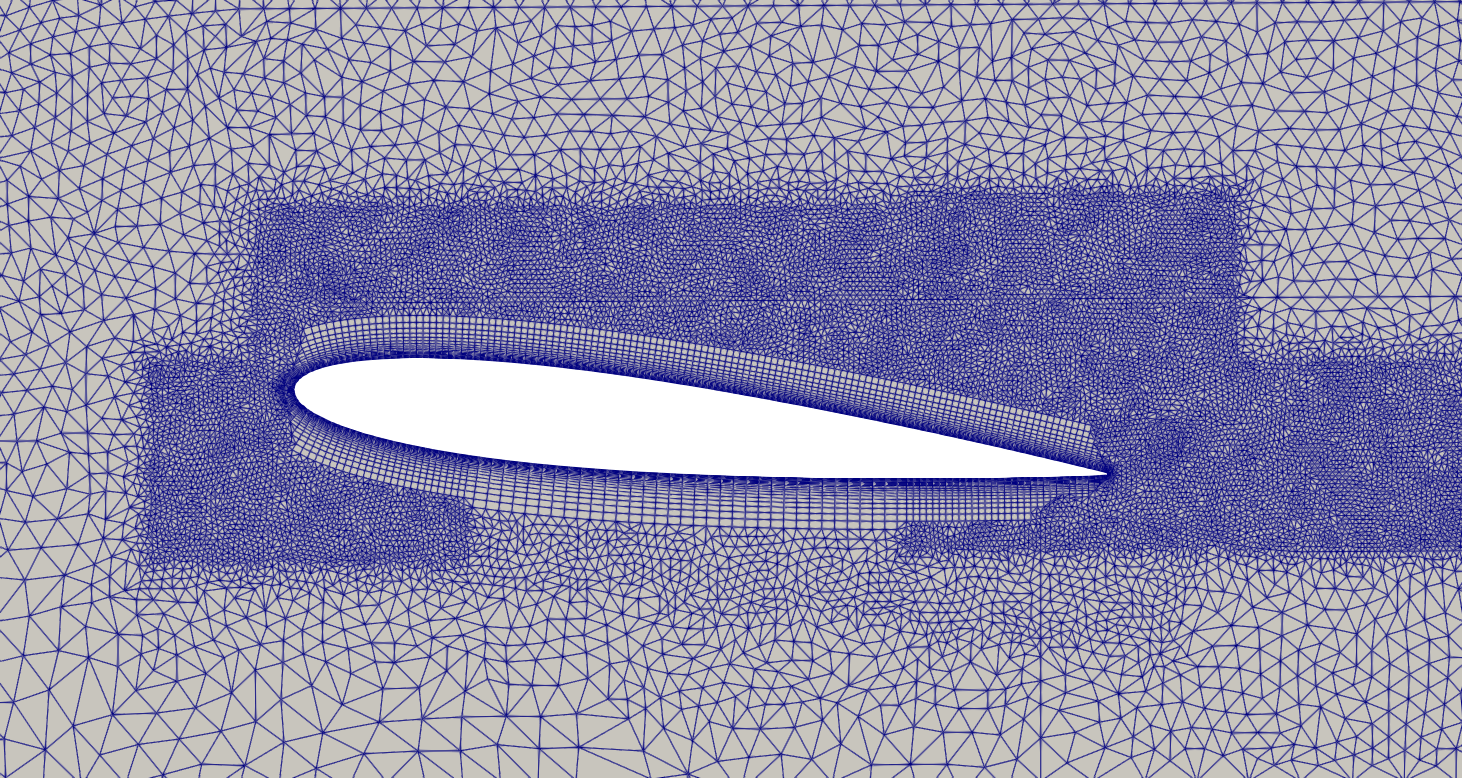
\includegraphics[width=1\textwidth]{figures/adapt_strat/zoomed/Mfa1_mesh.png}
		\caption{Mfa1\_nz50 mesh}
		\label{fig:Mfa1_mesh_zoomed}
	\end{subfigure}
	\begin{subfigure}[b]{0.7\textwidth}
		\centering
		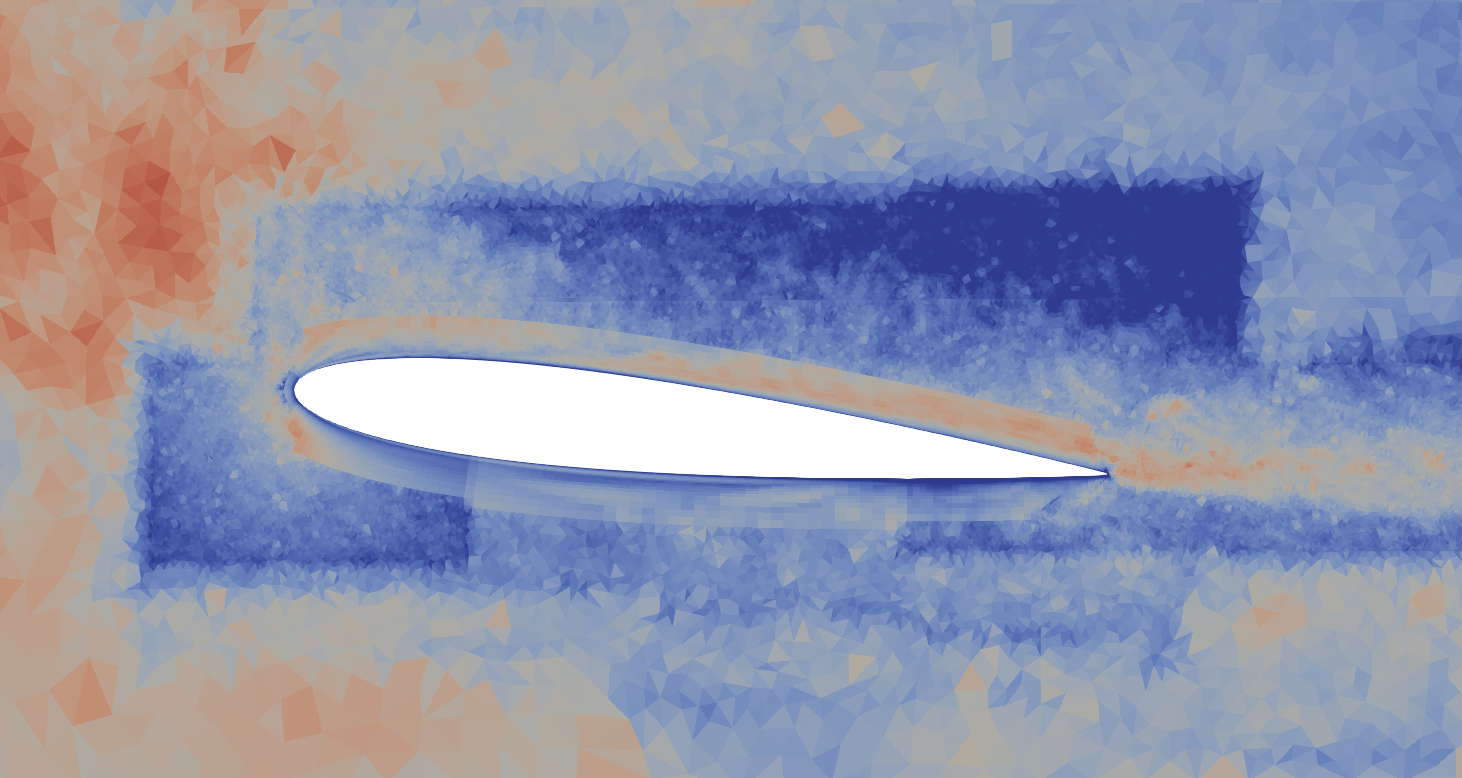
\includegraphics[width=1\textwidth]{figures/adapt_strat/zoomed/Mfa1_error.png}
		\caption{Mfa1\_nz50 estimated error}
		\label{fig:Mfa1_max_error_zoomed}
	\end{subfigure}
	\begin{subfigure}[b]{0.7\textwidth}
		\centering
		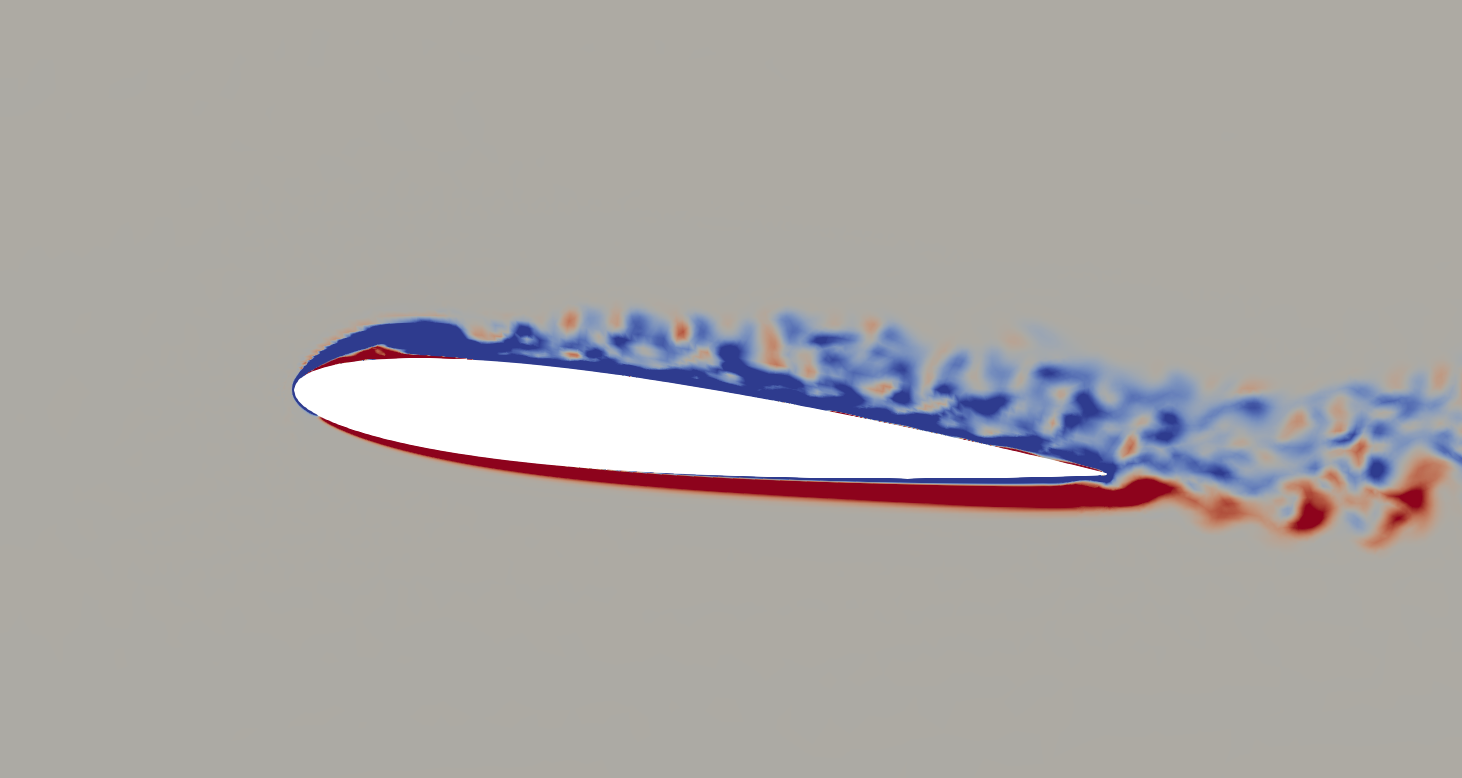
\includegraphics[width=1\textwidth]{figures/adapt_strat/zoomed/Mfa1_ph_210.png}
		\caption{Mfa1\_nz50 vorticity at $\psi=210^\circ$}
		\label{fig:Mfa1_vorticity_zoomed}
	\end{subfigure}
	\caption{Zoomed-in view for Mfa1\_nz50: mesh, estimated error and vorticity}
	\label{fig:Mfa1_zoomed}
\end{figure}



For a more quantitative comparison, we focus on pressure coefficient, $C_p$,  at different phases of interest including those around LEV formation. $C_p$ is shown in Figure \ref{fig:Cp_plots} at six phases for all adapted meshes. At $\psi=180^\circ$, we can see that flow has started to separate for all meshes apart from M0\_nz25. For $\psi=195^\circ$, Msa1\_nz50 shows a larger $C_p$ value as compared to the other meshes, with M0\_nz25 showing the lowest $C_p$. For $\psi=210^\circ$, LEV presence is seen for all meshes apart from the M0\_nz25 mesh. At $\psi=225^\circ$, LEV presence and flow separation is seen for all meshes, with some differences in separation location for Msa1\_nz50 as compared to Mza1\_nz50 and Mfa1\_nz50. Note that a different range of $C_p$ is used for each phase to highlight the differences. At
$\psi=270^\circ$ and $285^\circ$, marginal differences are seen in $C_p$ among different meshes, specifically at the geometric trailing edge where flow separation starts to occur. 

%%Cp plots

\begin{figure}[H]
\centering

\begin{subfigure}[b]{0.475\textwidth}
\centering
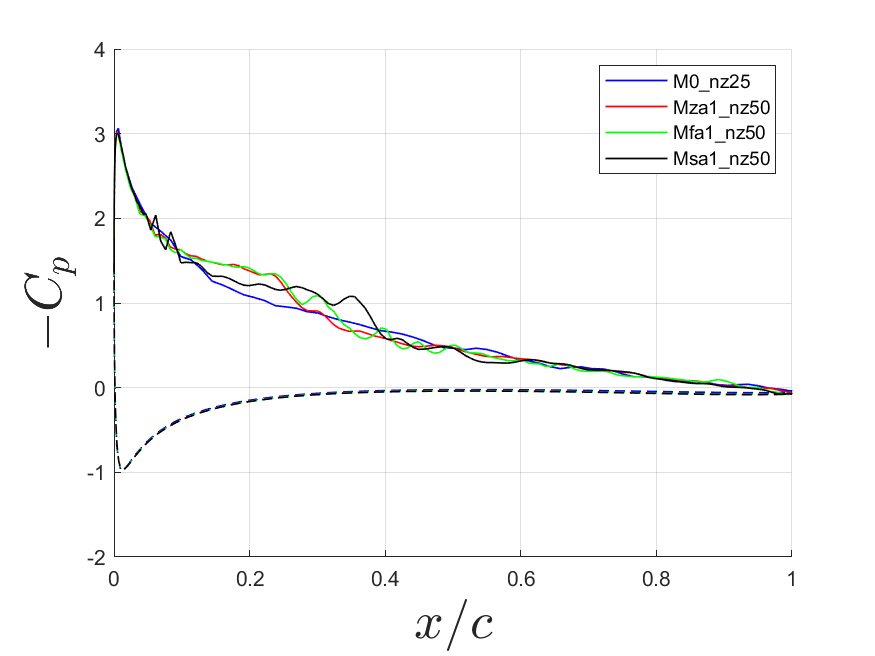
\includegraphics[width=1\textwidth]{figures/Results/Cp_plots/Cp_ph_180.png}
\caption{ $C_p$ at $\psi$ = $180^\circ$}
\label{fig:Cp_180}
\end{subfigure}
\begin{subfigure}[b]{0.475\textwidth}
\centering
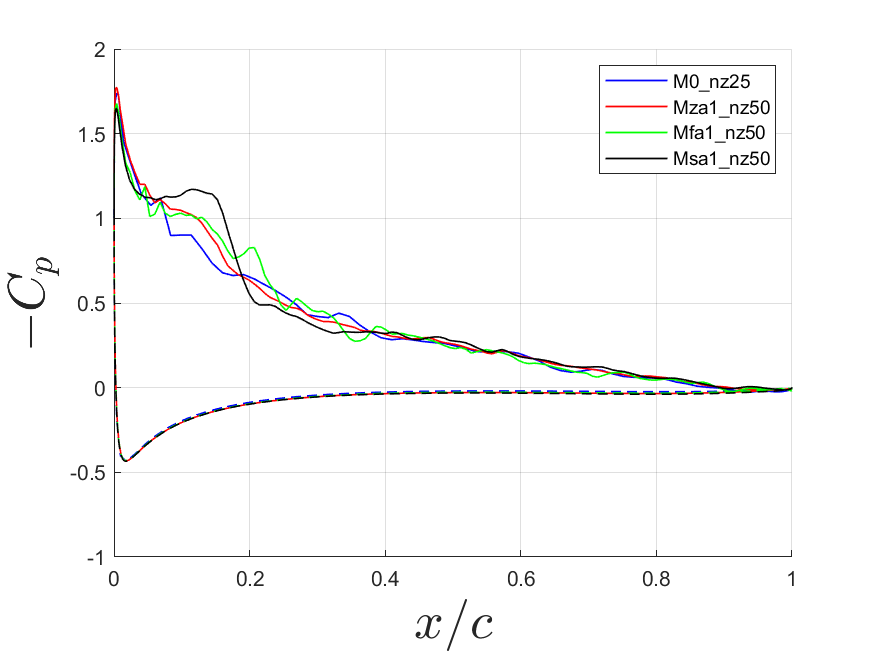
\includegraphics[width=1\textwidth]{figures/Results/Cp_plots/Cp_ph_195.png}
\caption{ $C_p$ at $\psi$ = $195^\circ$}
\label{fig:Cp_195}
\end{subfigure}
\begin{subfigure}[b]{0.475\textwidth}
\centering
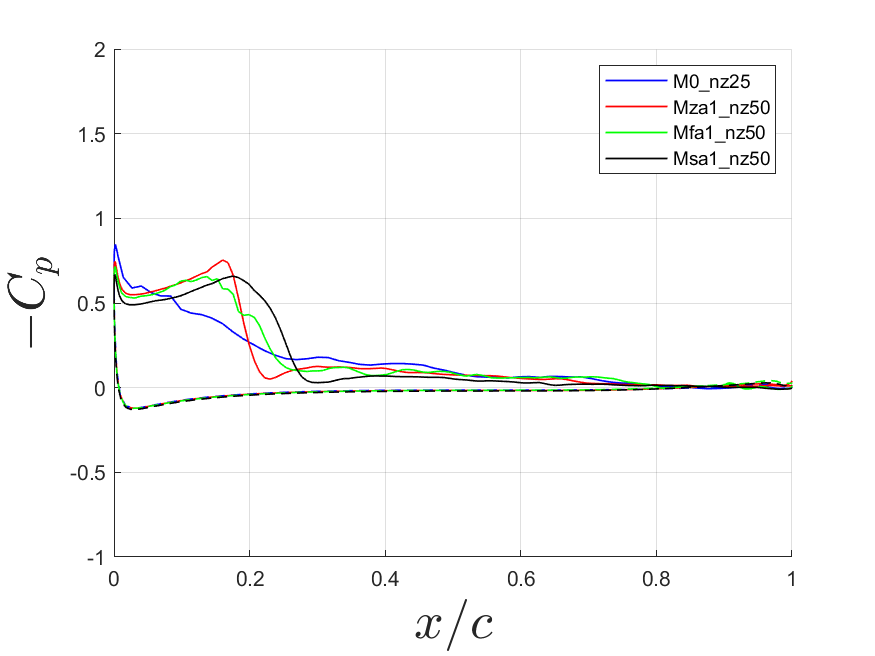
\includegraphics[width=1\textwidth]{figures/Results/Cp_plots/Cp_ph_210.png}
\caption{ $C_p$ at $\psi$ = $210^\circ$}
\label{fig:Cp_210}
\end{subfigure}
\begin{subfigure}[b]{0.475\textwidth}
\centering
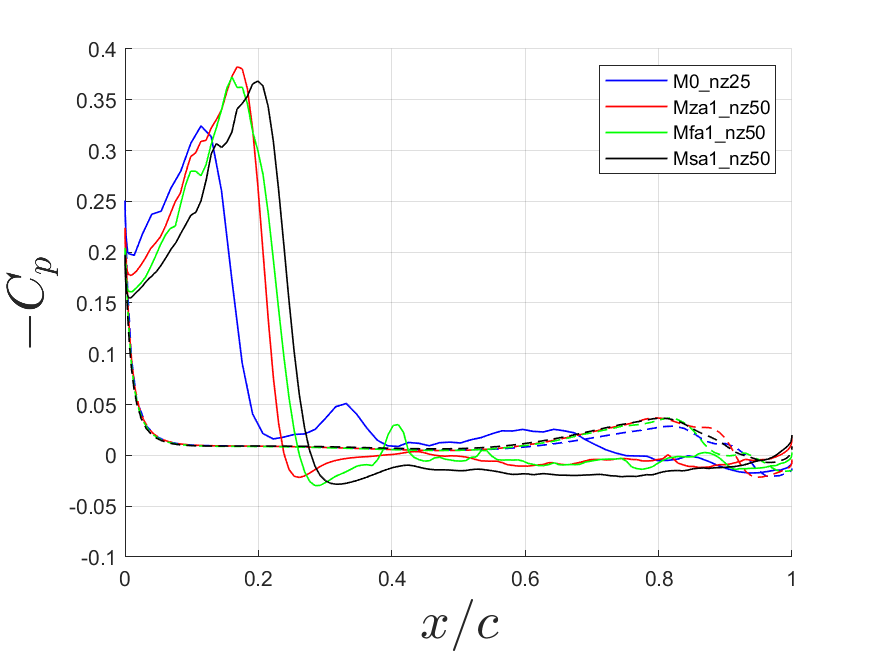
\includegraphics[width=1\textwidth]{figures/Results/Cp_plots/Cp_ph_225.png}
\caption{ $C_p$ at $\psi$ = $225^\circ$}
\label{fig:Cp_225}
\end{subfigure}
\begin{subfigure}[b]{0.475\textwidth}
\centering
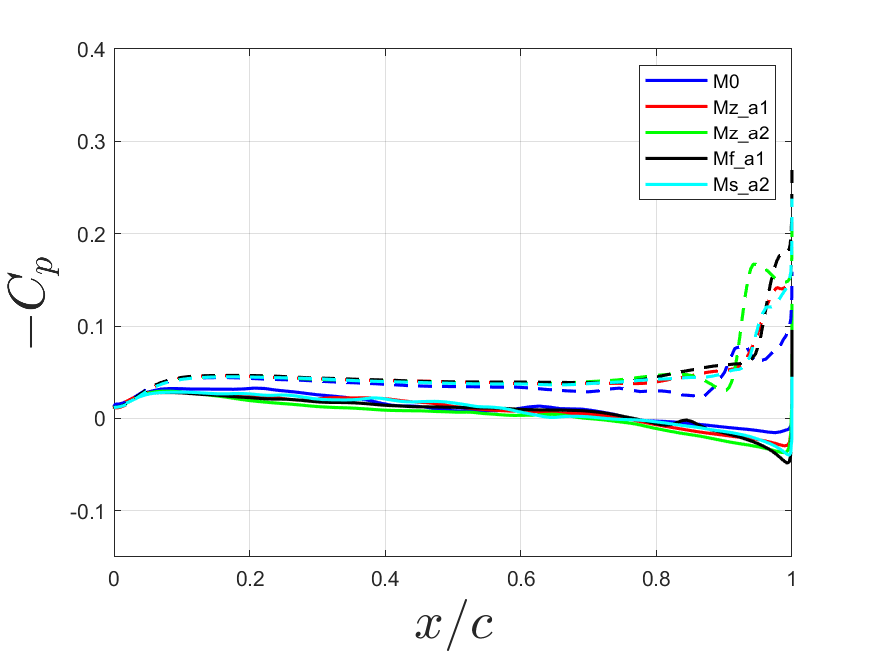
\includegraphics[width=1\textwidth]{figures/Results/Cp_plots/Cp_ph_270.png}
\caption{ $C_p$ at $\psi$ = $270^\circ$}
\label{fig:Cp_270}
\end{subfigure}
\begin{subfigure}[b]{0.475\textwidth}
\centering
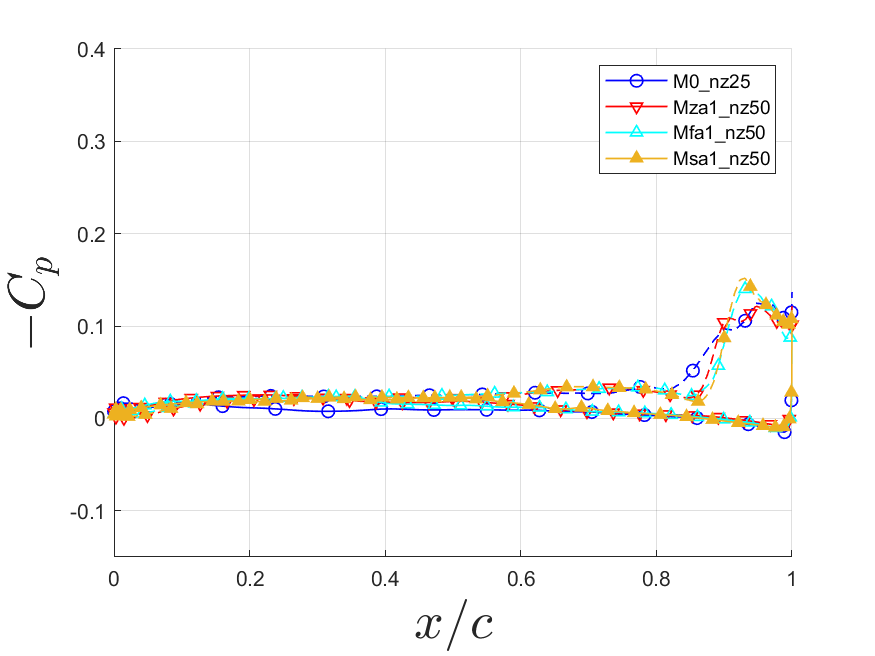
\includegraphics[width=1\textwidth]{figures/Results/Cp_plots/Cp_ph_285.png}
\caption{ $C_p$ at $\psi$ = $285^\circ$}
\label{fig:Cp_285}
\end{subfigure}
\caption{Pressure coefficient for different adaptive strategies/adapted meshes (data on the top/upper surface of airfoil is denoted by solid lines and on the bottom/lower surface by dashed lines)}
\label{fig:Cp_plots}
\end{figure}

In summary, mesh refinement/adaptation is necessary to perform accurate LES of complex aerodynamic flows. The above comparison among different adaptive strategies clearly indicates that the zonal-based refinement/adaptation strategy is the most appropriate for the current problem of interest involving surging airfoils. Thus, it is used in the following to construct a series of adapted meshes and demonstrate mesh convergence.